\documentclass[color=usenames,dvipsnames]{beamer}\usepackage[]{graphicx}\usepackage[]{color}
% maxwidth is the original width if it is less than linewidth
% otherwise use linewidth (to make sure the graphics do not exceed the margin)
\makeatletter
\def\maxwidth{ %
  \ifdim\Gin@nat@width>\linewidth
    \linewidth
  \else
    \Gin@nat@width
  \fi
}
\makeatother

\definecolor{fgcolor}{rgb}{0.345, 0.345, 0.345}
\newcommand{\hlnum}[1]{\textcolor[rgb]{0.686,0.059,0.569}{#1}}%
\newcommand{\hlstr}[1]{\textcolor[rgb]{0.192,0.494,0.8}{#1}}%
\newcommand{\hlcom}[1]{\textcolor[rgb]{0.678,0.584,0.686}{\textit{#1}}}%
\newcommand{\hlopt}[1]{\textcolor[rgb]{0,0,0}{#1}}%
\newcommand{\hlstd}[1]{\textcolor[rgb]{0.345,0.345,0.345}{#1}}%
\newcommand{\hlkwa}[1]{\textcolor[rgb]{0.161,0.373,0.58}{\textbf{#1}}}%
\newcommand{\hlkwb}[1]{\textcolor[rgb]{0.69,0.353,0.396}{#1}}%
\newcommand{\hlkwc}[1]{\textcolor[rgb]{0.333,0.667,0.333}{#1}}%
\newcommand{\hlkwd}[1]{\textcolor[rgb]{0.737,0.353,0.396}{\textbf{#1}}}%
\let\hlipl\hlkwb

\usepackage{framed}
\makeatletter
\newenvironment{kframe}{%
 \def\at@end@of@kframe{}%
 \ifinner\ifhmode%
  \def\at@end@of@kframe{\end{minipage}}%
  \begin{minipage}{\columnwidth}%
 \fi\fi%
 \def\FrameCommand##1{\hskip\@totalleftmargin \hskip-\fboxsep
 \colorbox{shadecolor}{##1}\hskip-\fboxsep
     % There is no \\@totalrightmargin, so:
     \hskip-\linewidth \hskip-\@totalleftmargin \hskip\columnwidth}%
 \MakeFramed {\advance\hsize-\width
   \@totalleftmargin\z@ \linewidth\hsize
   \@setminipage}}%
 {\par\unskip\endMakeFramed%
 \at@end@of@kframe}
\makeatother

\definecolor{shadecolor}{rgb}{.97, .97, .97}
\definecolor{messagecolor}{rgb}{0, 0, 0}
\definecolor{warningcolor}{rgb}{1, 0, 1}
\definecolor{errorcolor}{rgb}{1, 0, 0}
\newenvironment{knitrout}{}{} % an empty environment to be redefined in TeX

\usepackage{alltt}
%\documentclass[color=usenames,dvipsnames,handout]{beamer}

%\usepackage[roman]{../pres1}
\usepackage[sans]{../pres1}




\IfFileExists{upquote.sty}{\usepackage{upquote}}{}
\begin{document}



\begin{frame}[plain]
  \begin{center}
    {\huge Distance sampling \par}
    \vspace{0.5cm}
%    { \Large March 25, 2019} \\
    {\color{RoyalBlue} \rule{\textwidth}{1pt}}
    \vfill
    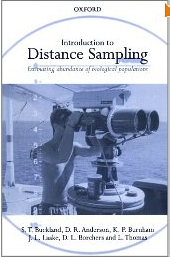
\includegraphics[height=5.5cm,keepaspectratio]{figs/book1} %\hfill
    \hspace{0.5cm}
      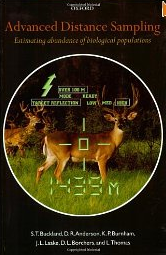
\includegraphics[height=5.5cm,keepaspectratio,trim = 0mm
        0mm 0mm 0mm, clip]{figs/book2}
  \end{center}
\end{frame}




\section{Introduction}



\begin{frame}
  \frametitle{Estimating abundance}
  \large
  Abundance estimation is often accomplished using this equation:
  \[
    \hat{N} = \frac{n}{\hat{p}}
  \]
  \begin{itemize}
    \item $N$ is abundance (population size)
%      \footnote{Density is just $\hat{D} = \hat{N}/A$}
    \item $n$ is the number of individuals detected
    \item $\hat{p}$ is an estimate of detection probability: The probability
      of detecting an individual
  \end{itemize}
  \pause
  \vfill
%  \Large
  \centering
  \bf
  Most methods differ in how they estimate $p$ \\
\end{frame}






\begin{frame}
  \frametitle{Estimating abundance}
  \large
  {\bf Challenges}
  \begin{itemize}
    \item<1-> Detection probability is rarely constant
    \item<2-> It is a function of: %\dots
    \begin{itemize}
      \large
      \item Age
      \item Sex
      \item Habitat
      \item \alert{Distance}
    \end{itemize}
%    \item<3-> Special sampling methods are required to estimate
  \end{itemize}
%  \vspace{0.5cm}
%  \uncover<3->{In distance sampling, $p$ is defined as the
%    probability of detecting an \emph{individual}, given its distance to the
%    transect. }

%  \uncover<3->{
%    In distance sampling, detection probability differs for every
%    individual.
%    }
\end{frame}







\begin{frame}
  \frametitle{Distance Sampling}
%  \begin{block}
  \large
  {\bf Basic idea} \\
  \begin{itemize}
  \item<1-> $p_i$ is the probability of detecting individual $i$ at
    distance $x_i$.
  \item<2-> Since every individual in the population has a different
    detection probability, we replace $p$ with the {\it average}
    detection probability: $\bar{p}$
  \item<3-> The equation is now: \\
    \[
      \hat{N} = \frac{n}{\hat{\bar{p}}}
    \]
  \end{itemize}
%  \end{block}
%  \pause
%  \begin{block}
  \vspace{0.1cm}
  \uncover<4->{{\bf Advantages of distance sampling}} \\
    \begin{itemize}
      \item<5-> Population size can be estimated from a single survey
      \item<6-> Explicit link between population size and density
    \end{itemize}
%  \end{block}
\end{frame}




\begin{frame}
  \frametitle{Design}
  \Large
  \begin{itemize}%[<+->]
    \item Randomly place line transects or points throughout the study
      area
    \item Record the distance to each animal detected
  \end{itemize}
  \vspace{0.5cm}
  \begin{columns}
    \begin{column}{0.5\textwidth}
      {\centering Line transects \par}
      \includegraphics[width=\textwidth]{figs/Fig9-7}
    \end{column}
    \begin{column}{0.5\textwidth}
      {\centering Point transects \par}
      \includegraphics[width=\textwidth]{figs/Fig9-9}
    \end{column}
  \end{columns}
\end{frame}





% \begin{frame}
%   \frametitle{Conventional Distance Sampling}
%   \begin{block}{\bf Same as it ever was---almost}
%     \begin{itemize}%[<+->]
%       \item<1-> {\Large $E[C] = Np$ } % $N = \frac{C}{p}$}
% %      \item<2-> Except, $p_c$ and $p_a$ are assumed to be known
% %      \item<2-> $p_c = a/A$ and $p_a = 1$
%       \item<2-> But, detection probability ($p$) is a function of distance
%       \item<3-> So, $p$ is \alert{average} detection probability
%     \end{itemize}
%     \uncover<4>{
%     \Large
% %    \begin{columns}
% %      \begin{column}{2cm}
%         \begin{equation*}
%           \hat{N} = \frac{C}{\color{Red} \hat{p}}
%           \label{eq:dsN1}
%         \end{equation*}
% %      \end{column}
%       % \pause
% %      \begin{column}{2cm}
% %        \begin{equation*}
% %          \hat{N_s} = \frac{C}{\color{Red} \hat{p_d}}
% %          \label{eq:dsN1}
% %        \end{equation*}
% %      \end{column}
% %    \end{columns}
%     }
%   \end{block}
% \end{frame}










\section{Line transects}



\begin{frame}
  \frametitle{Line transects}
  \centering
  \includegraphics[width=0.8\textwidth]{figs/Fig9-1} \\
  In line transect sampling, it is common to record the radial
  distance and bearing, rather than the perpendicular
  distance. However, the analysis must be conducted on the
  perpendicular distance data. \\
\end{frame}


\begin{frame}
  \frametitle{Real design}
  \begin{columns}
    \begin{column}{0.6\textwidth}
      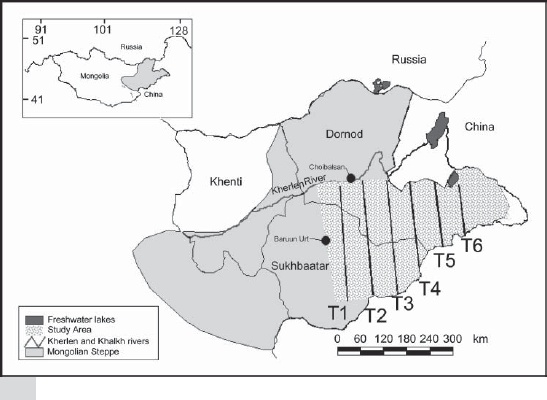
\includegraphics[width=\textwidth]{figs/Kirk}
    \end{column}
    \begin{column}{0.4\textwidth}
      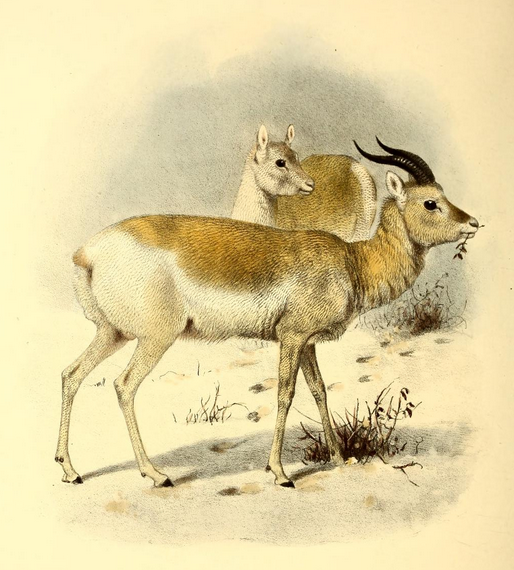
\includegraphics[width=\textwidth]{figs/Book_of_antelopes_(1894)_Gazella_gutturosa}
    \end{column}
  \end{columns}
\end{frame}



\begin{frame}
  \frametitle{Line transects}
  \begin{columns}
    \begin{column}{0.4\textwidth}
      \centering
      \normalsize
      \begin{tabular}{lc}
        \hline
        \multicolumn{2}{c}{Data} \\
        \hline
        Animal & Distance ($x$) \\
        \hline
        1 & 4.4 \\
        2 & 25.3 \\
        3 & 41.8 \\
        4 & 3.1 \\
        5 & 78.5 \\
        \vdots \\
        $n$ & 4.4 \\
        \hline
      \end{tabular}
    \end{column}
    \begin{column}{0.6\textwidth}
      \centering
      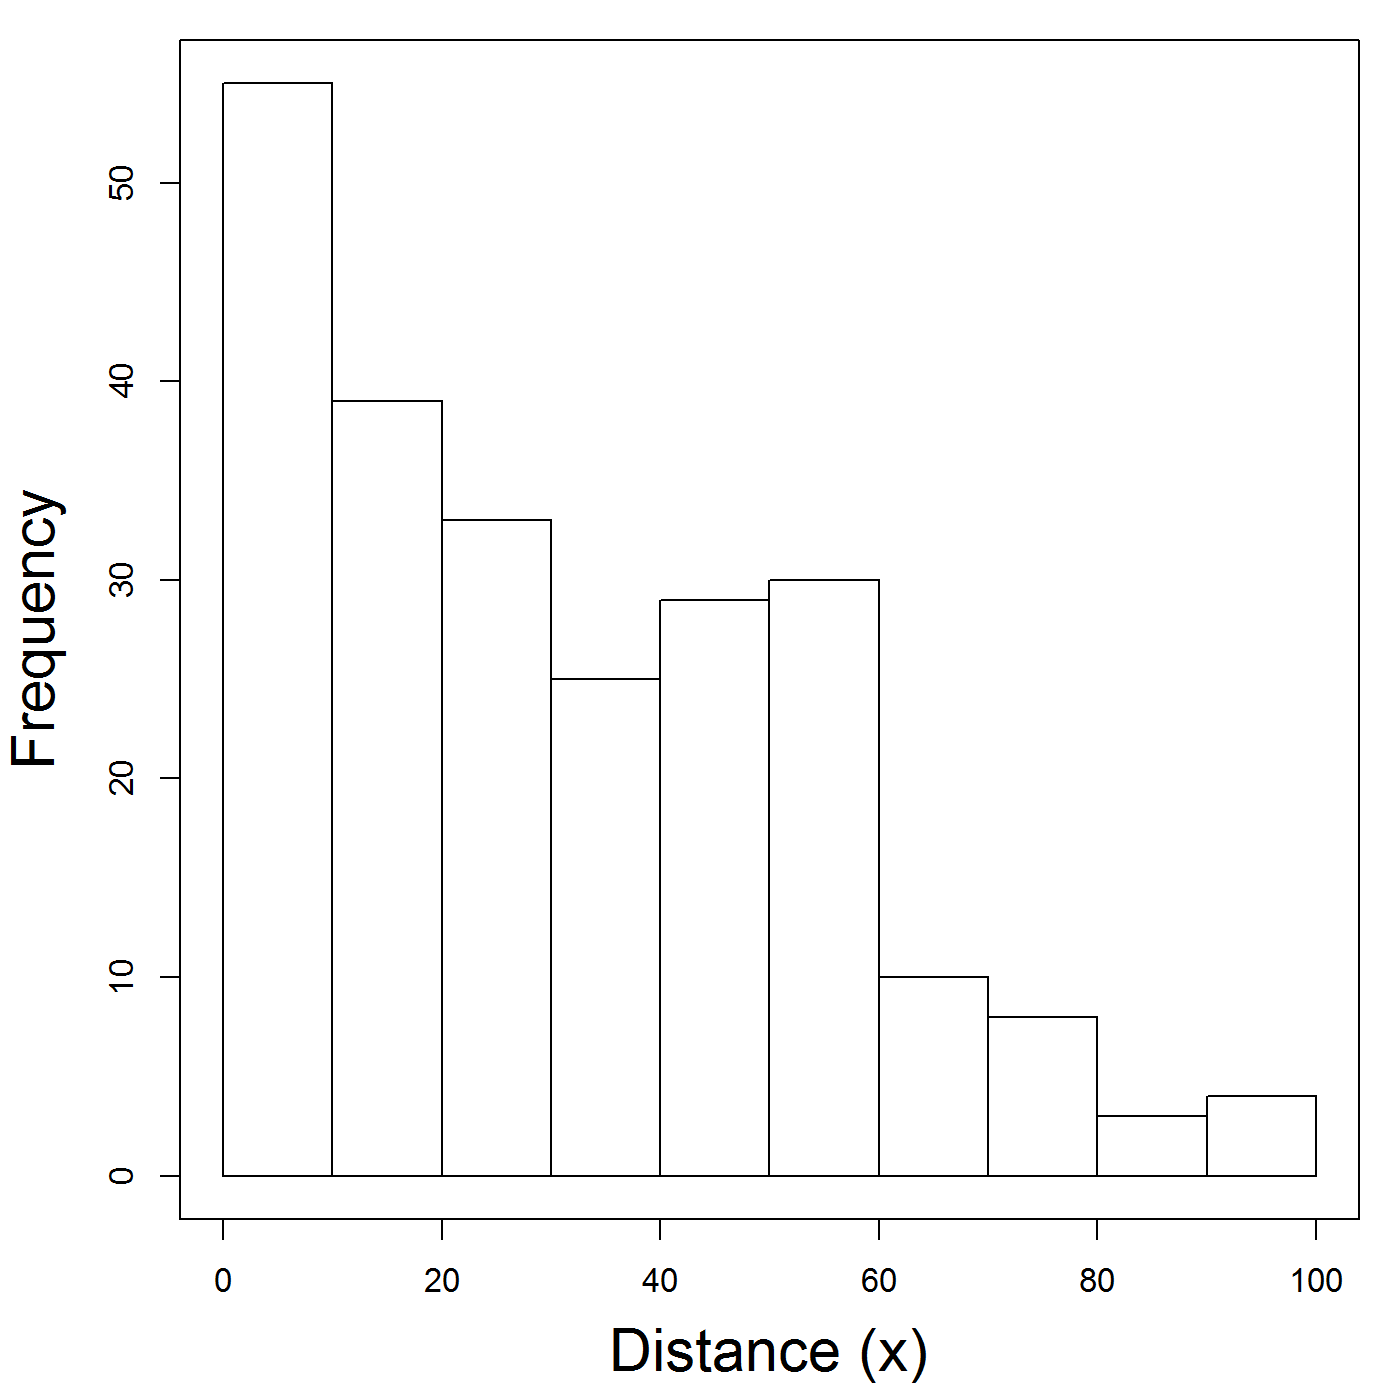
\includegraphics[width=5cm]{figs/example1}
    \end{column}
  \end{columns}

\end{frame}



\begin{frame}
  \frametitle{Estimating $\bar{p}$, average detection probability}
  \large
  \begin{itemize}
    \item<1-> Fit a detection function, $\mathrm{g}(x)$, to the data
      \begin{itemize}
        \item Assume $\mathrm{g}(0) = 1$
        \item Half-normal, hazard-rate, negative exponential, etc...
%  is a good one, $\mathrm{g}(x) = \exp(-x^2/(2\sigma^2))$
      \end{itemize}
    \item<2-> Assume individuals are ``uniformly'' distributed with
      respect to the transect (valid under random sampling)
    \item<3-> $\bar{p}$ is then the proportion of the area under the
      detection function.
    \end{itemize}
    \includegraphics<1->[width=\textwidth]{figs/detfuns}
\end{frame}






\begin{frame}
  \frametitle{Computing $\bar{p}$, average detection probability}
\begin{center}
  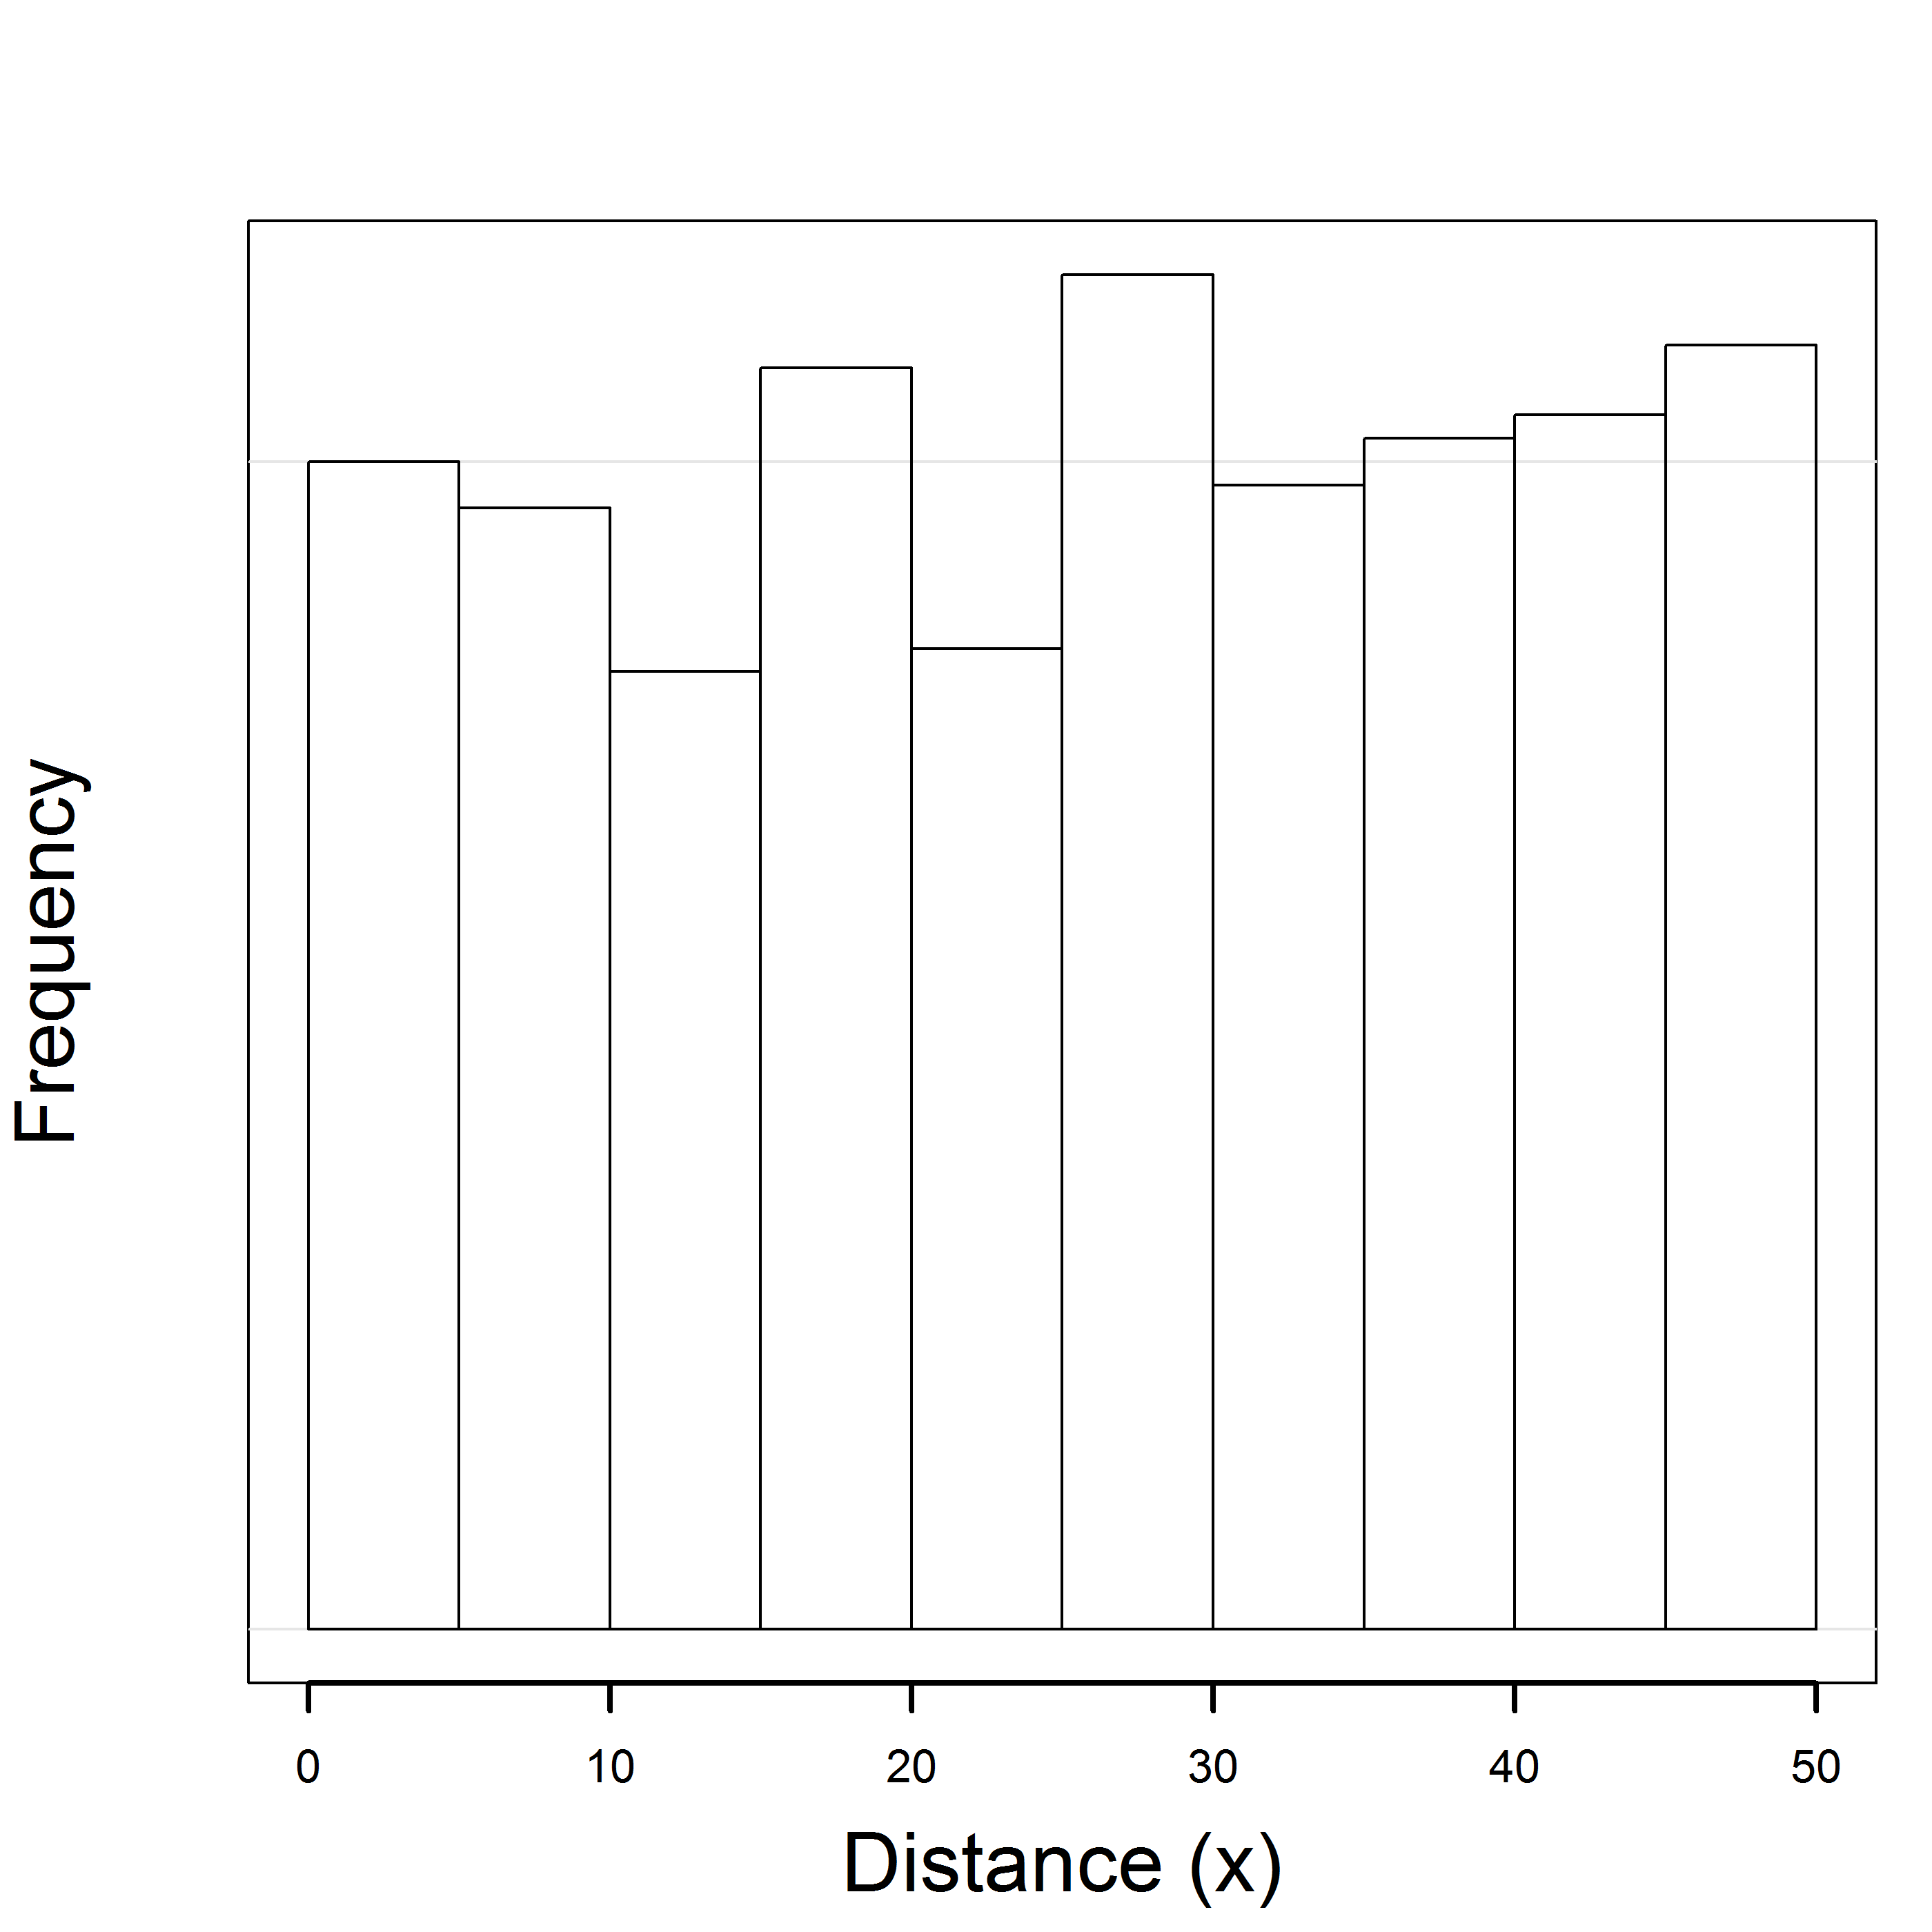
\includegraphics[width=7cm]{figs/detfun0-0}
\end{center}
\end{frame}



\begin{frame}
  \frametitle{Computing $\bar{p}$, average detection probability}
\begin{center}
  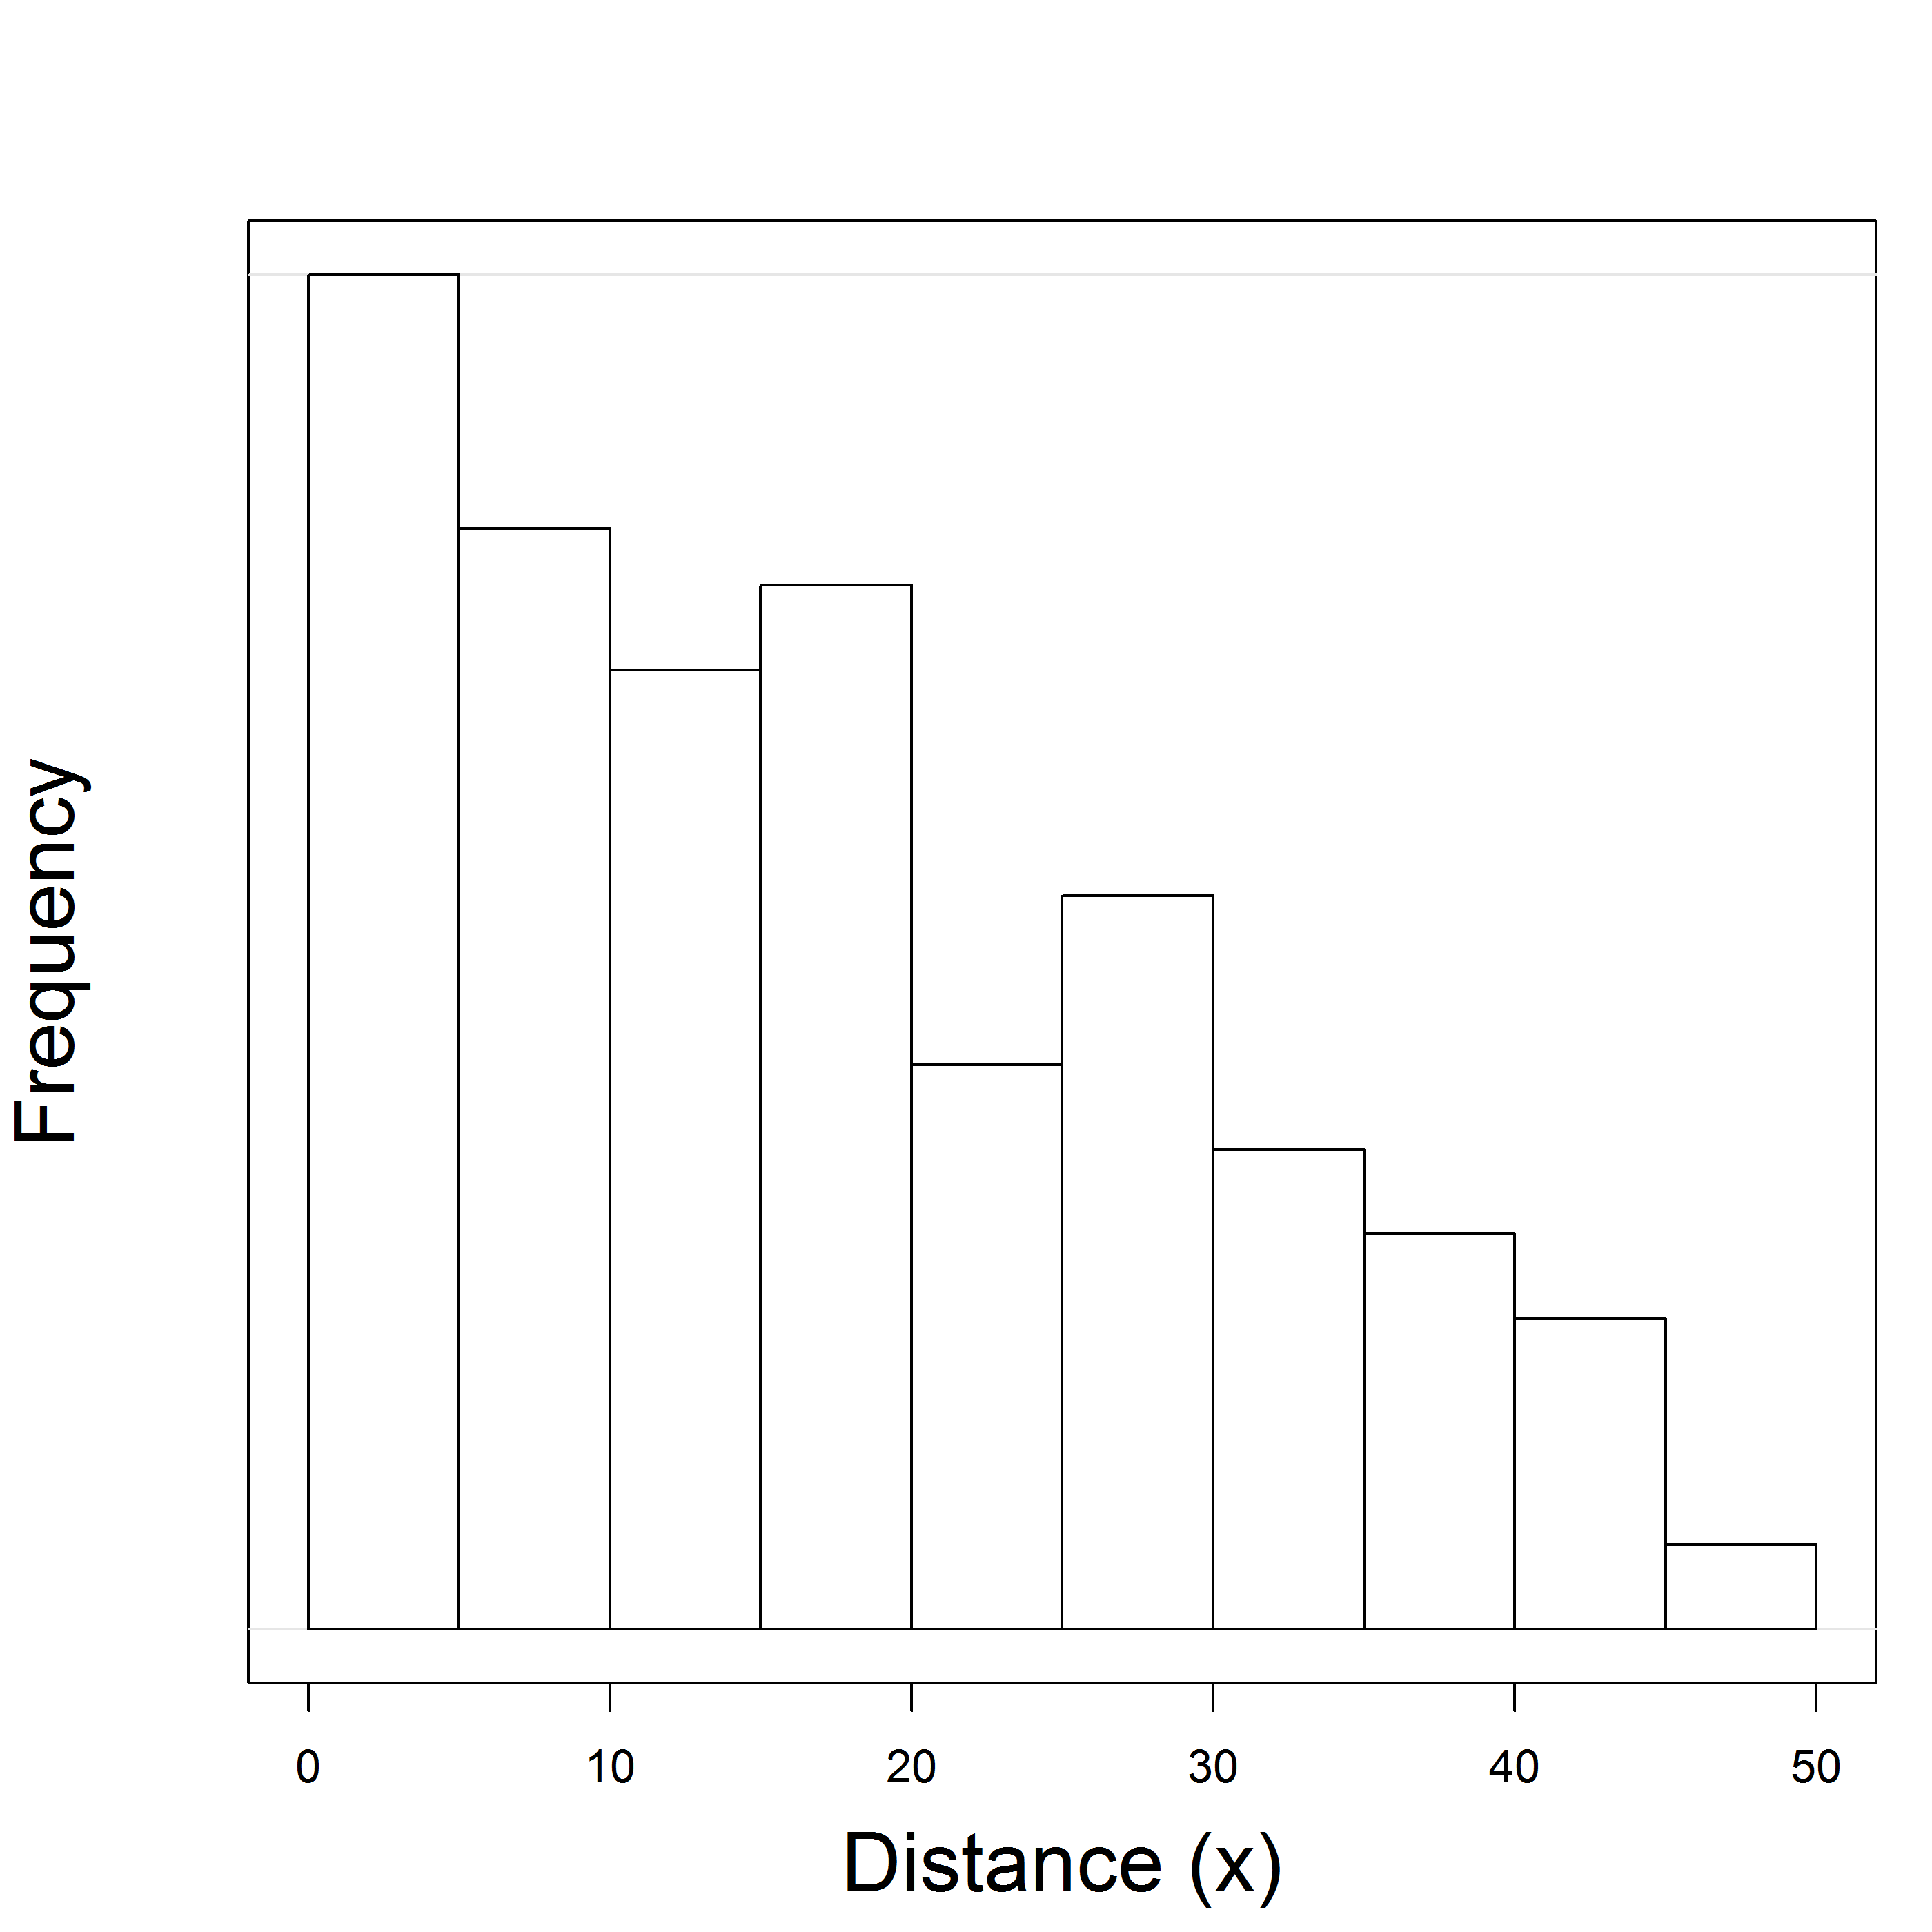
\includegraphics[width=7cm]{figs/detfun0-1}
\end{center}
\end{frame}




\begin{frame}
  \frametitle{Computing $\bar{p}$, average detection probability}
\begin{center}
  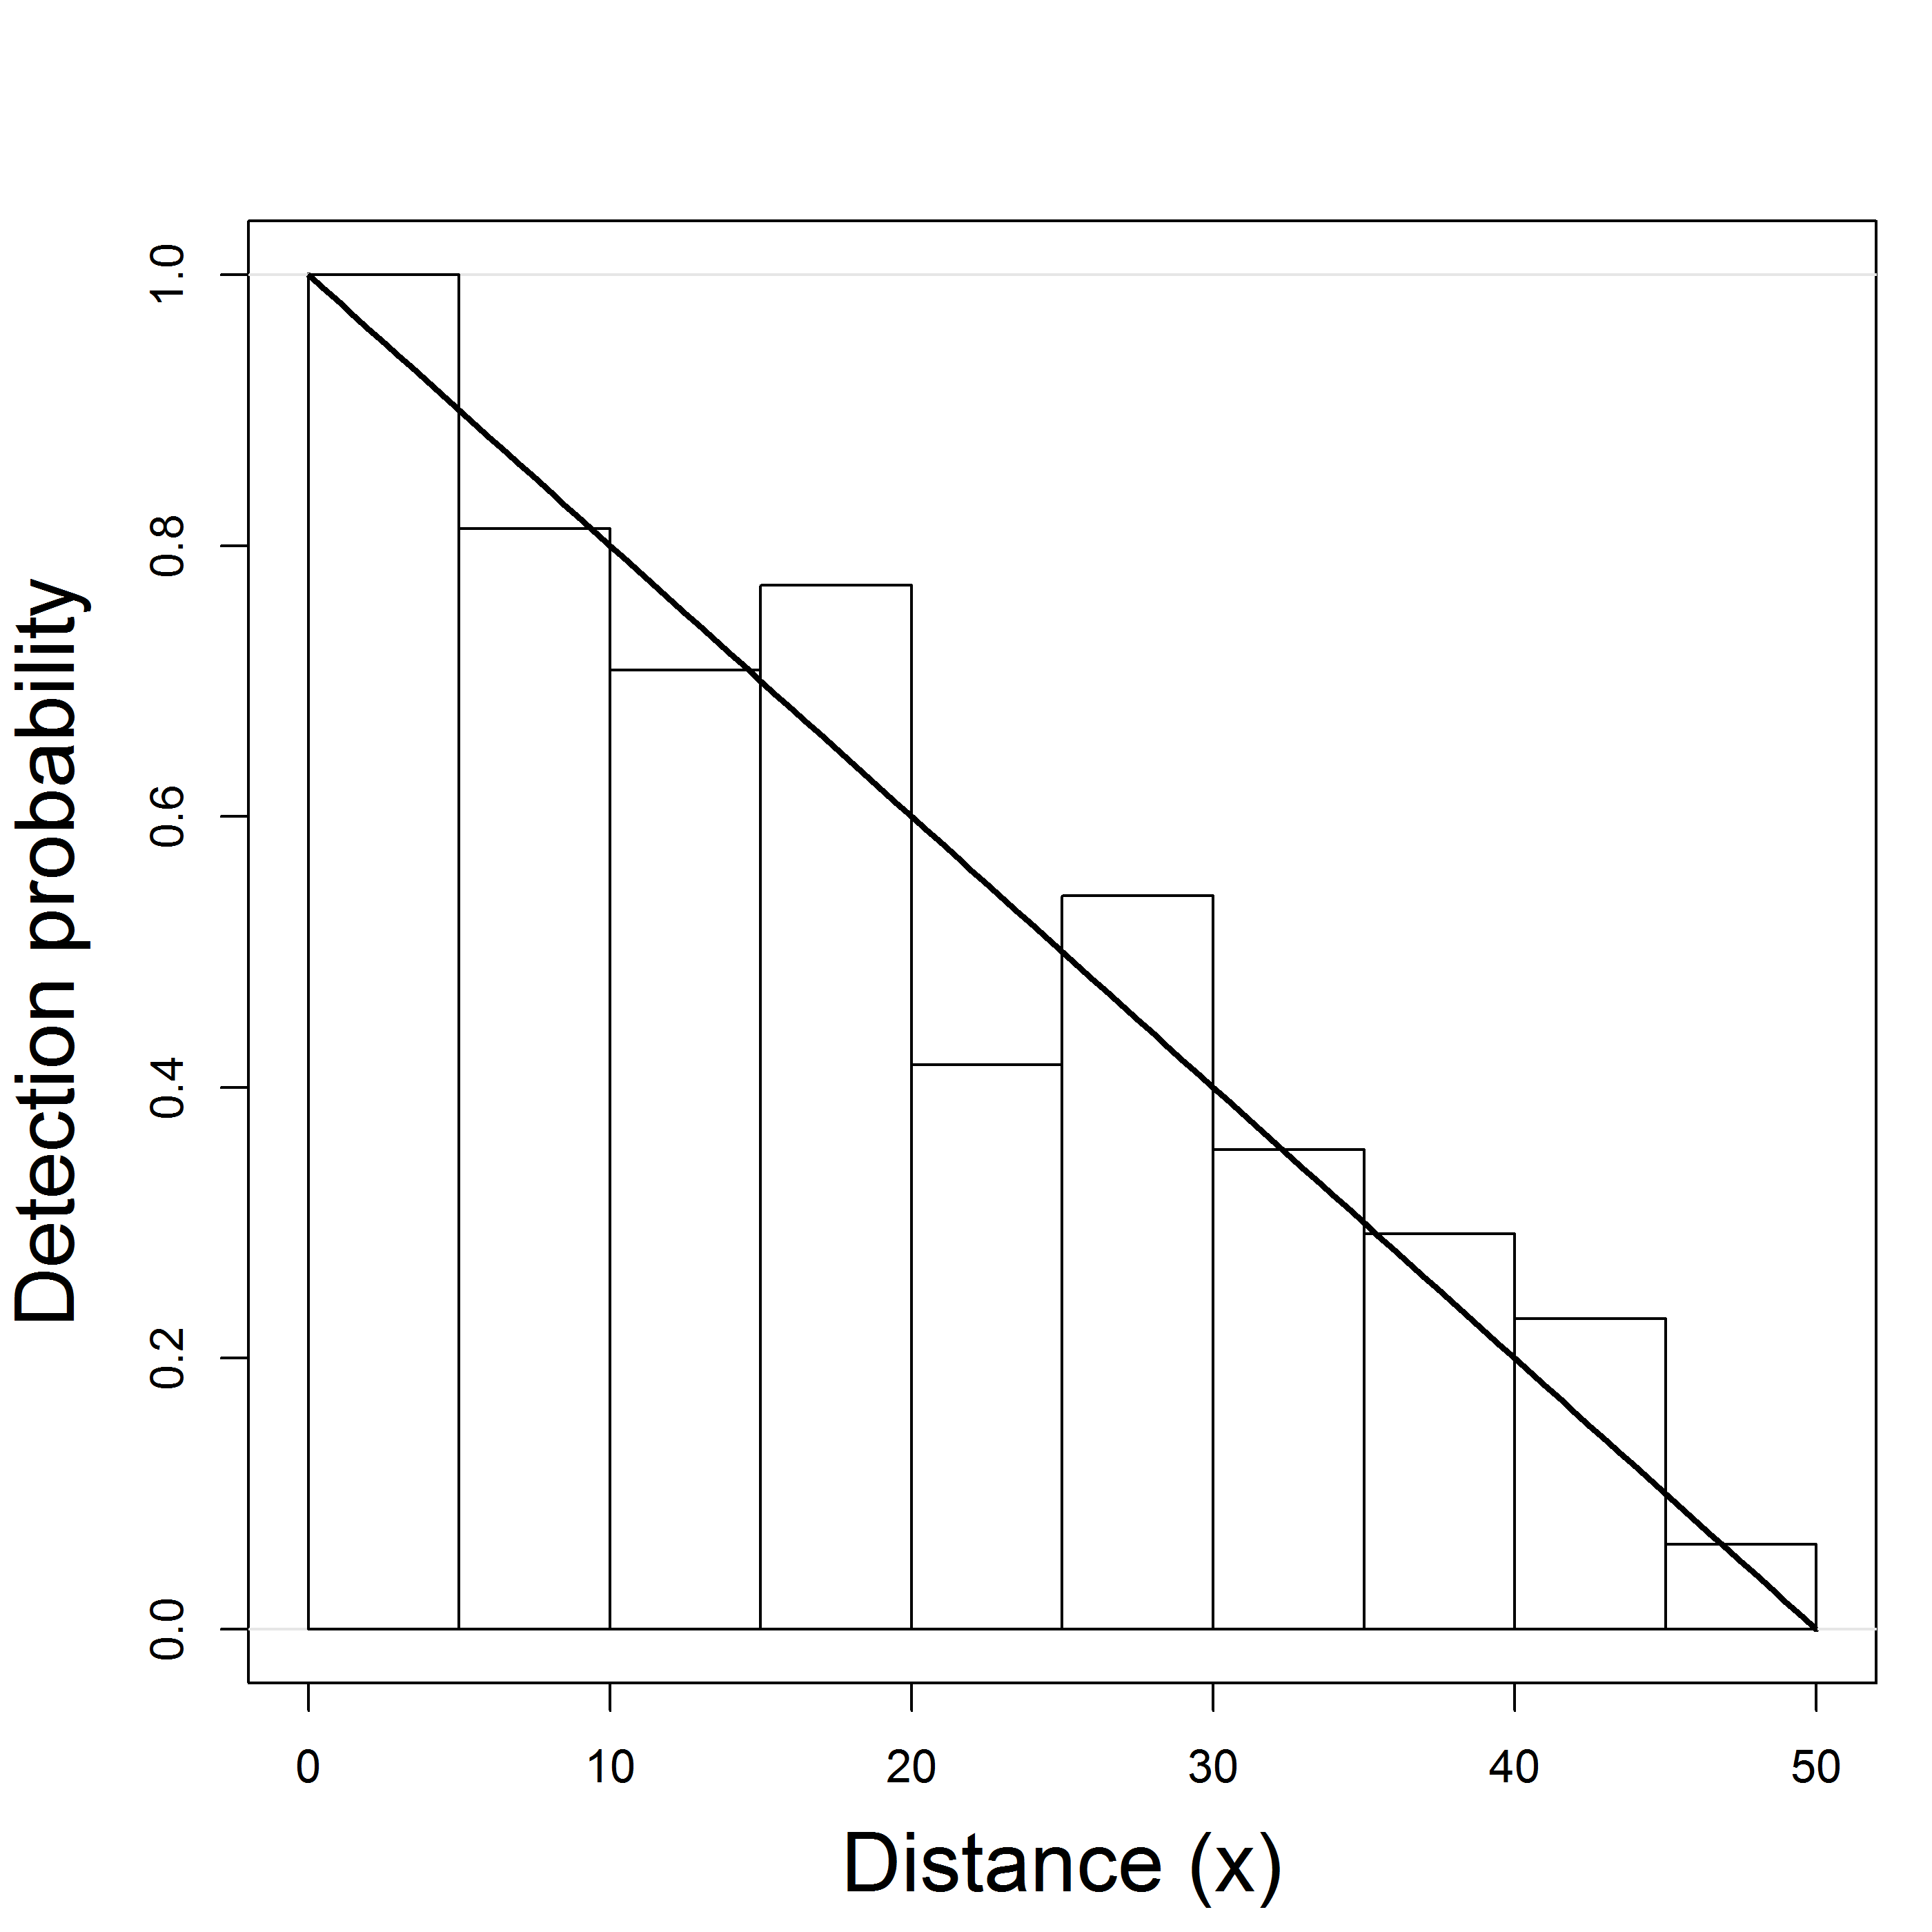
\includegraphics[width=7cm]{figs/detfun0-2}
\end{center}
\end{frame}




\begin{frame}
  \frametitle{Computing $\bar{p}$, average detection probability}
\begin{center}
  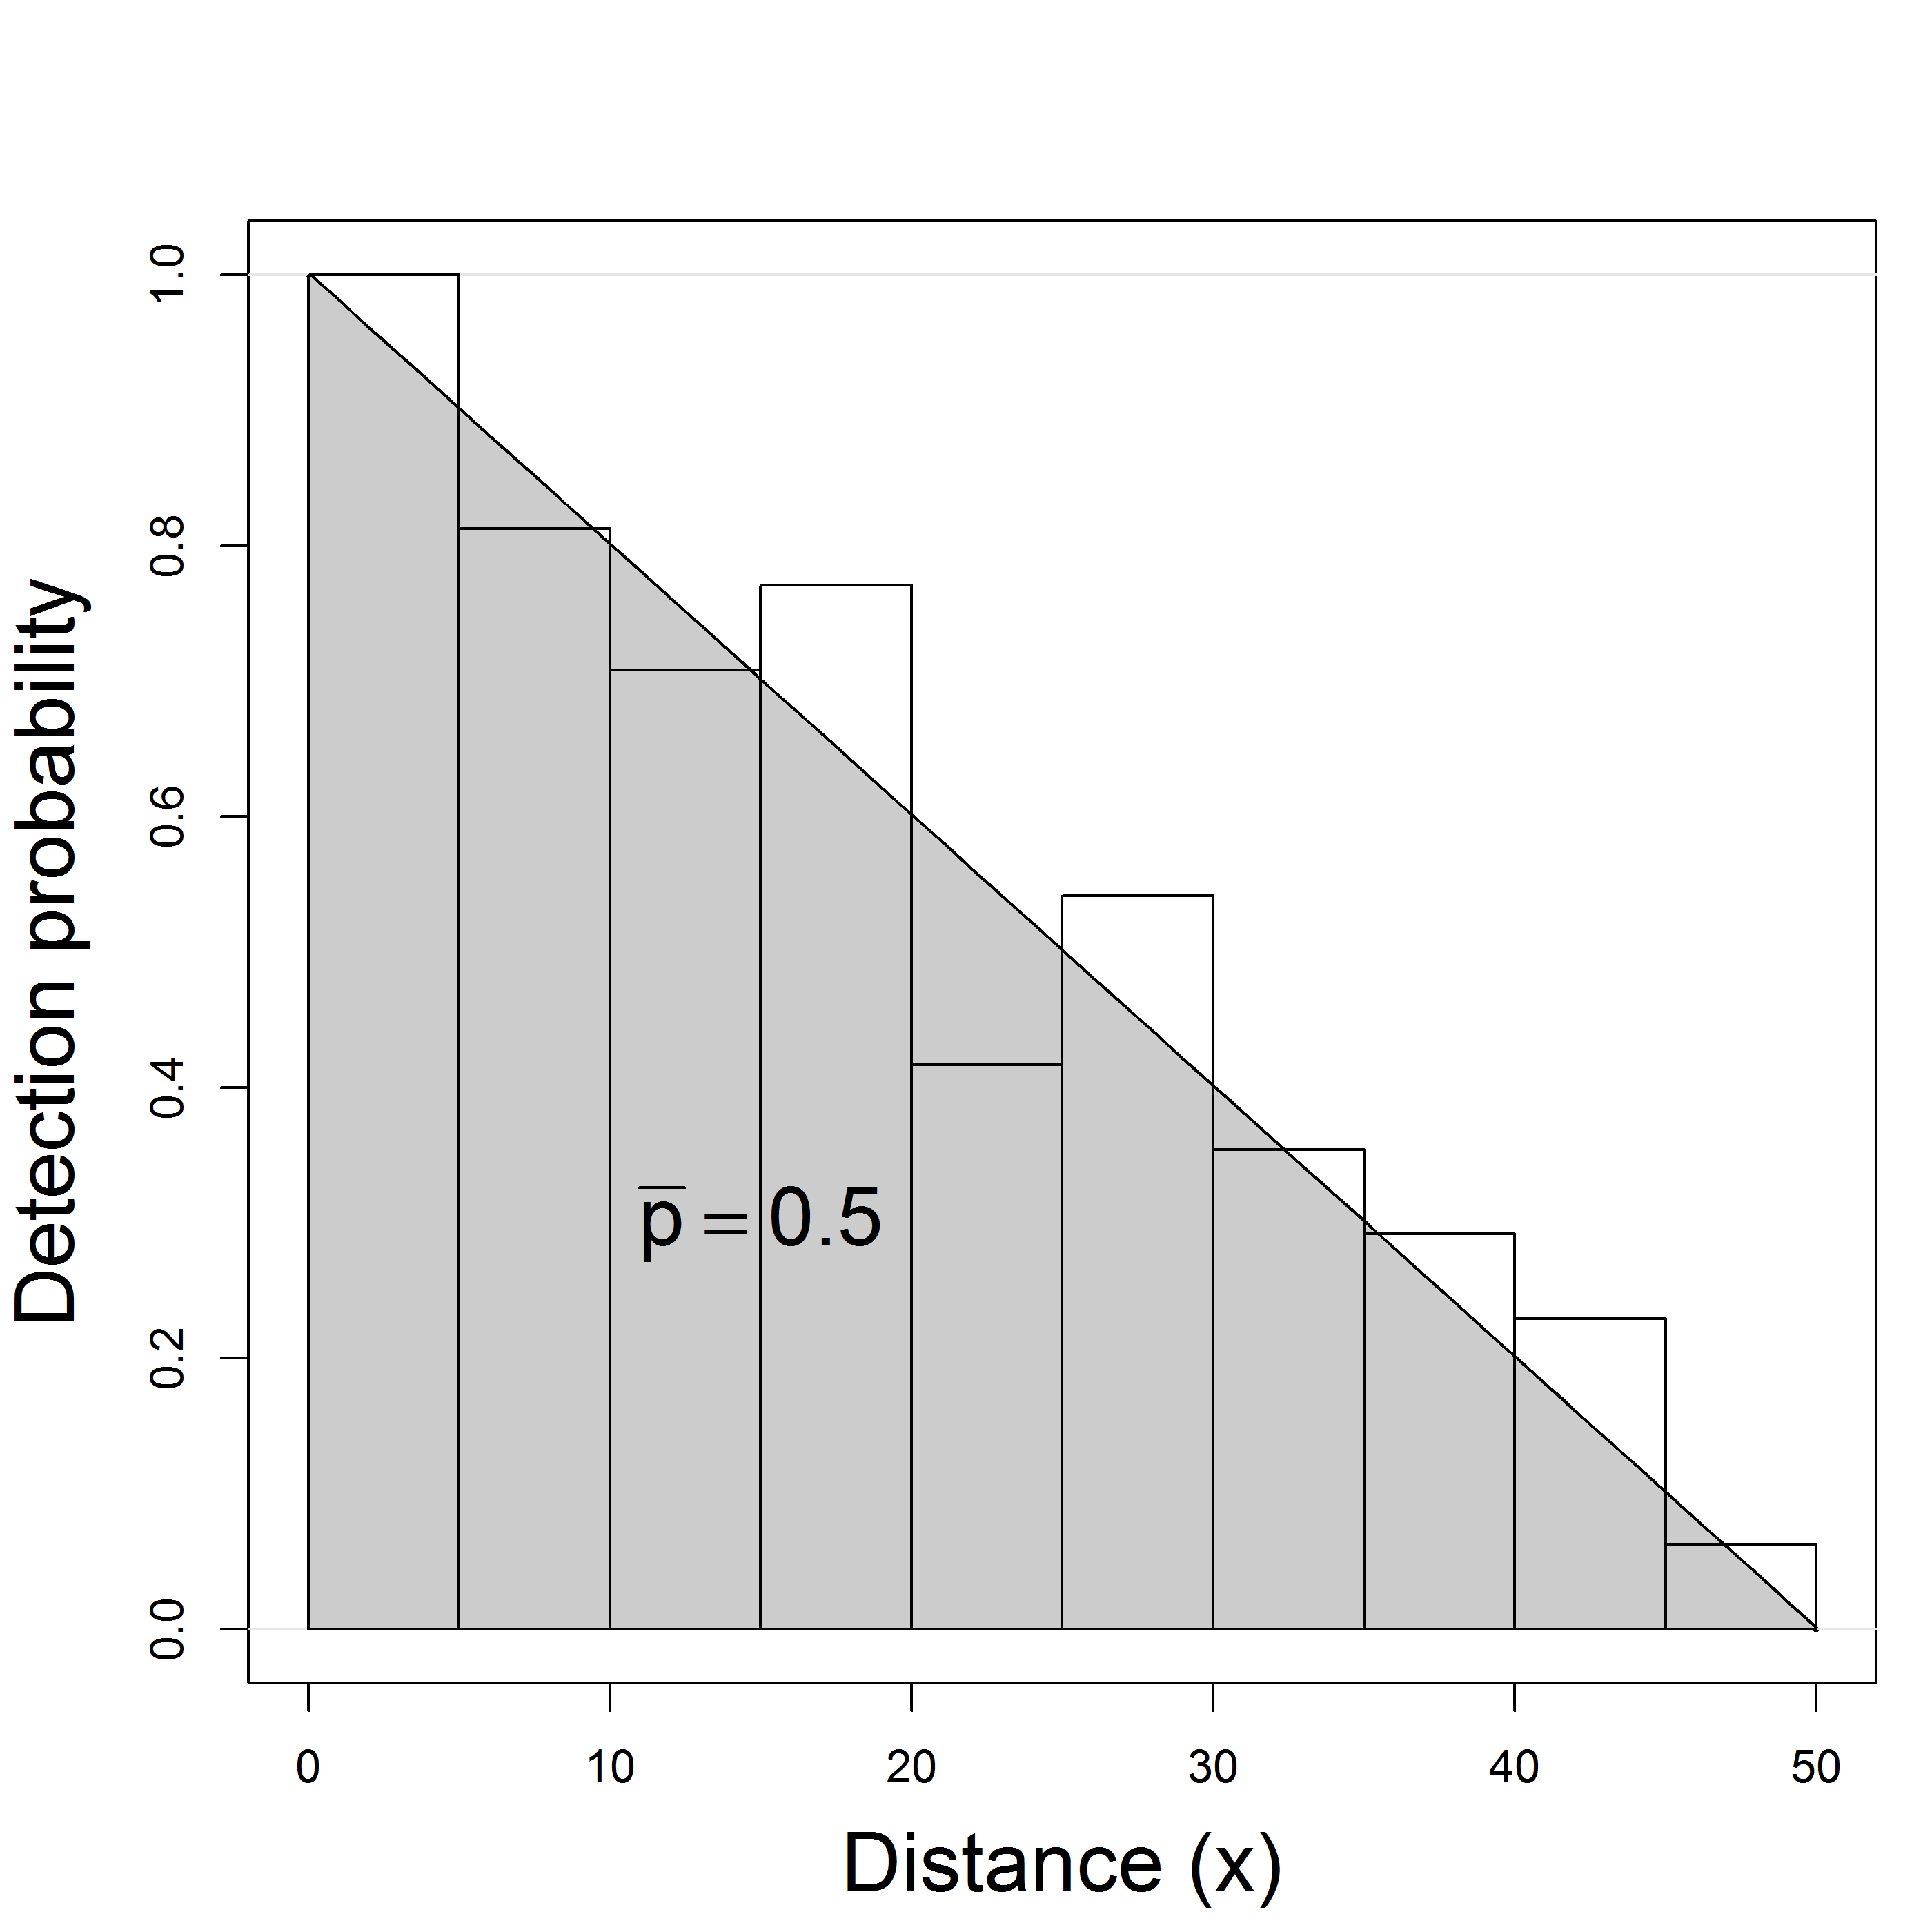
\includegraphics[width=7cm]{figs/detfun0-3}
\end{center}
\end{frame}




\begin{frame}
  \frametitle{Computing $\bar{p}$, average detection probability}
\begin{center}
  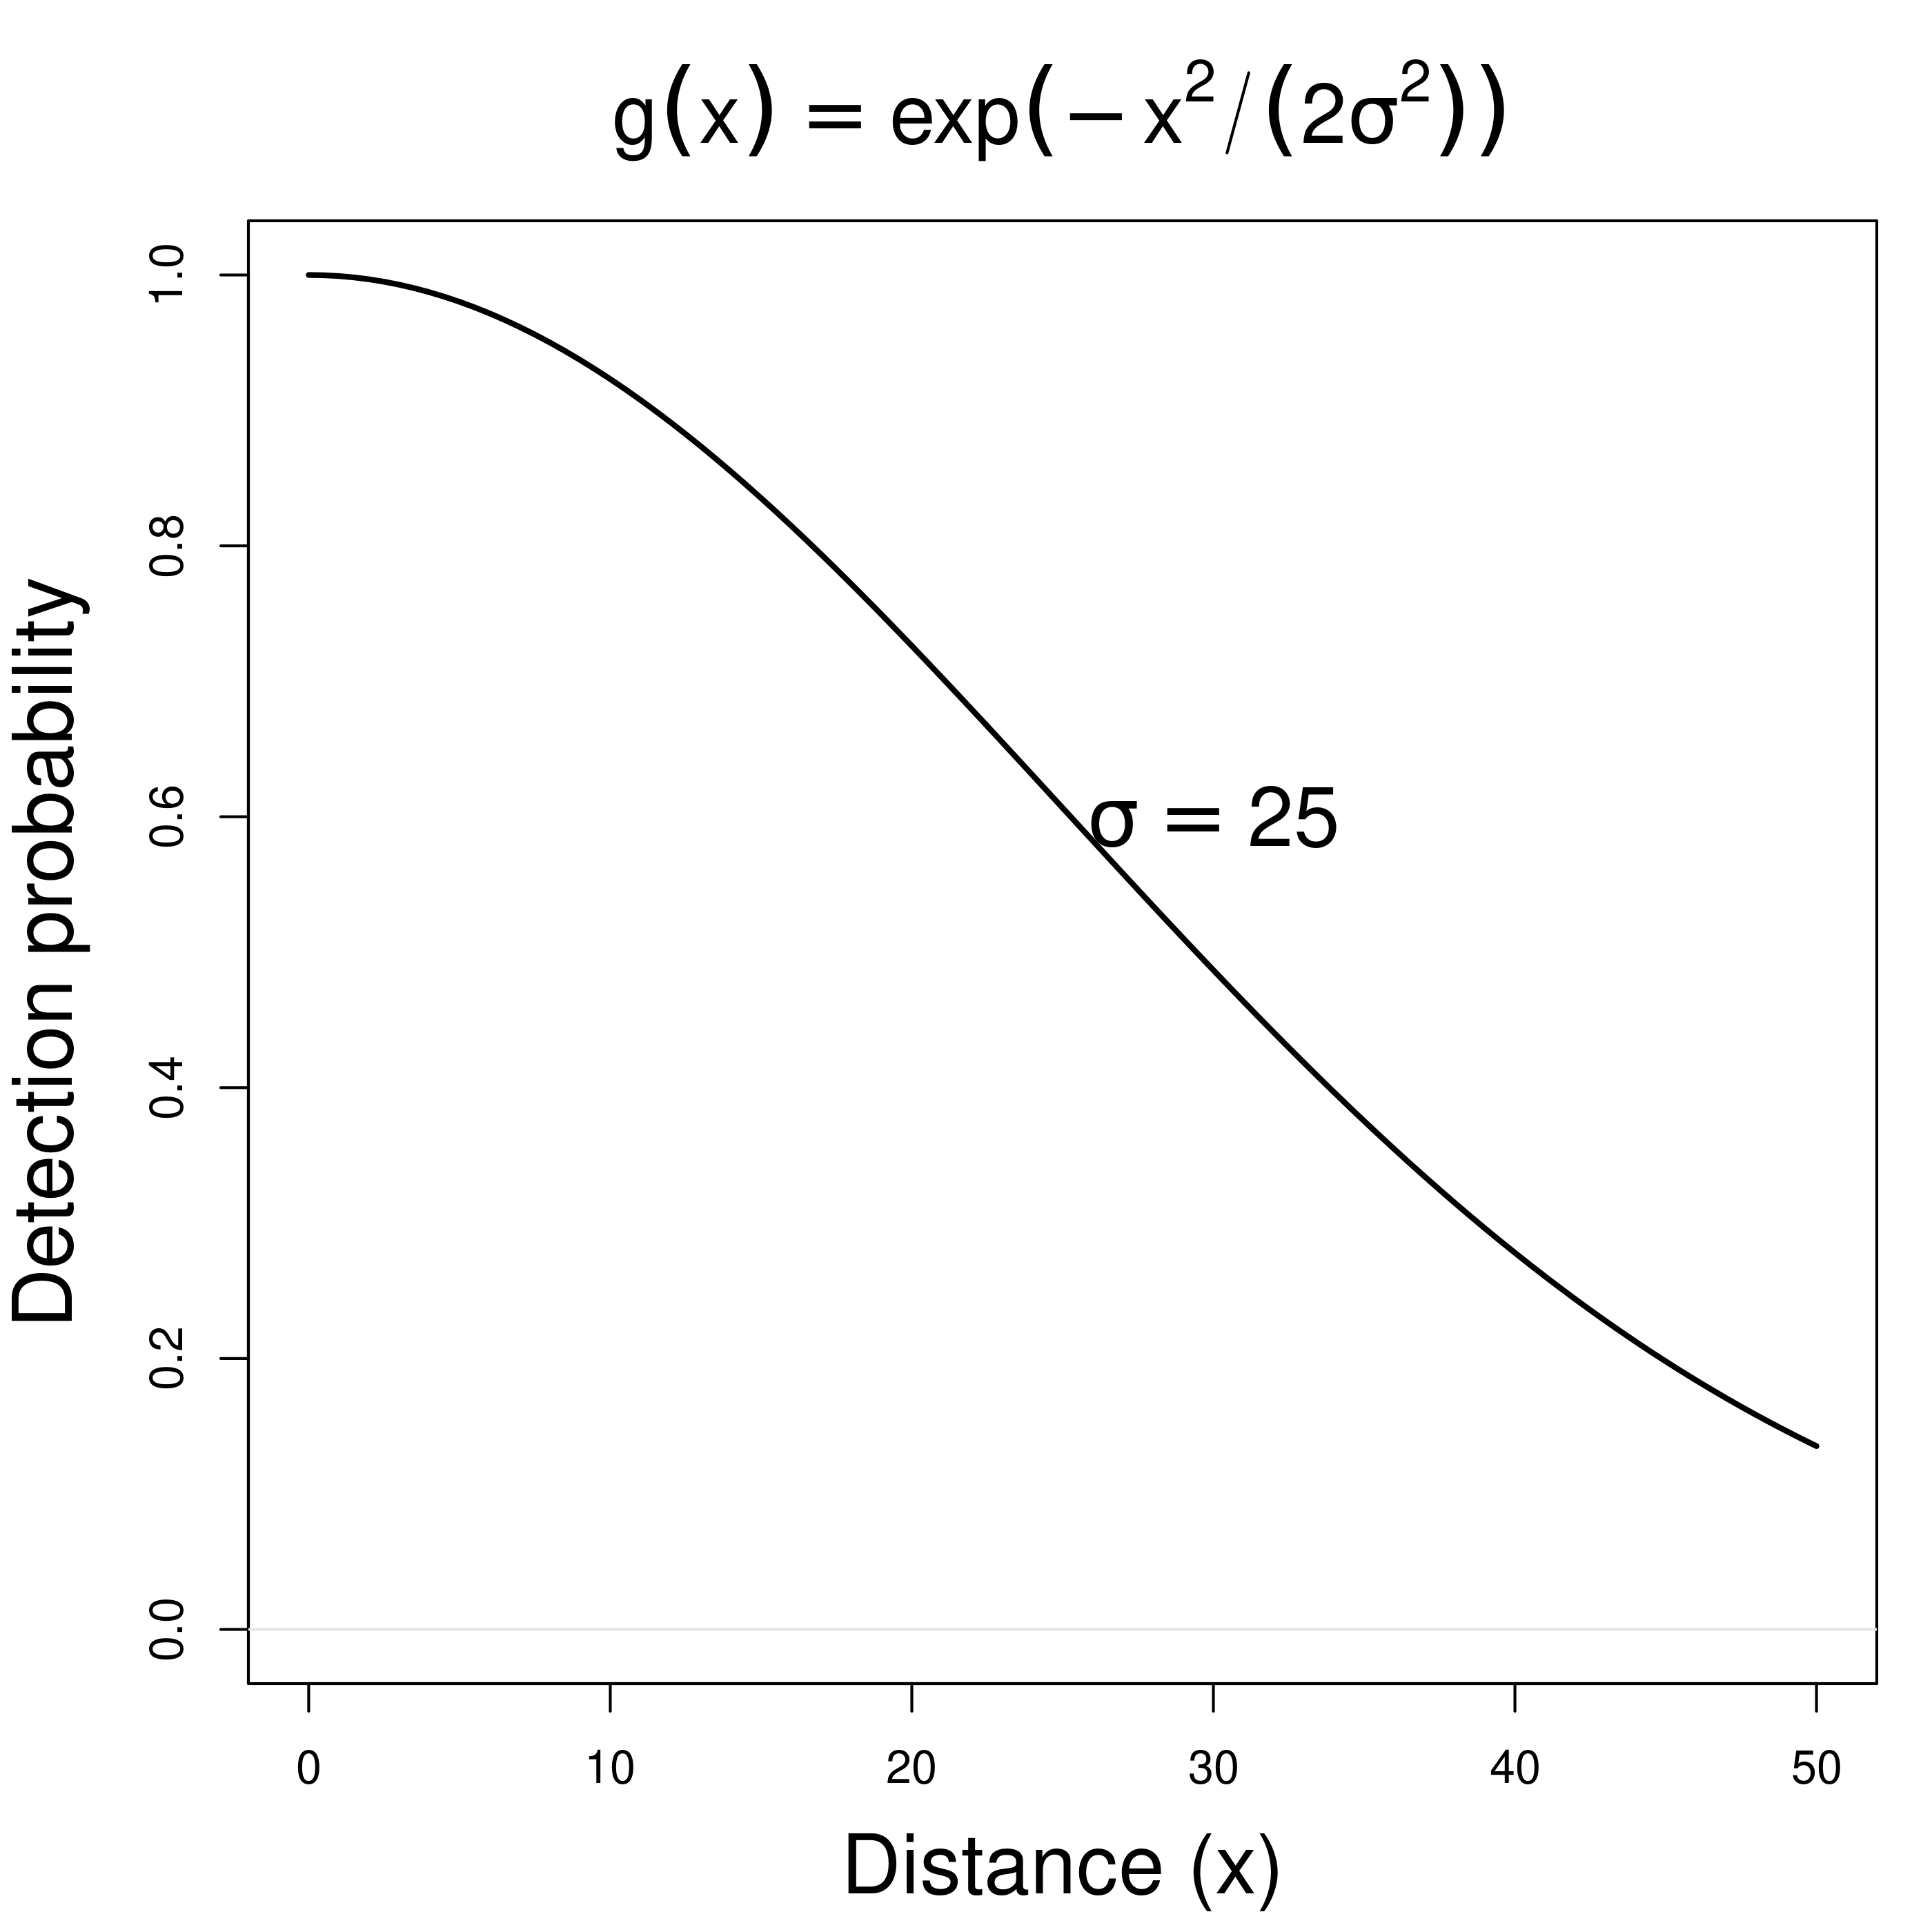
\includegraphics[width=7cm]{figs/detfun1}
\end{center}
\end{frame}




\begin{frame}
  \frametitle{Computing $\bar{p}$, average detection probability}
\begin{center}
  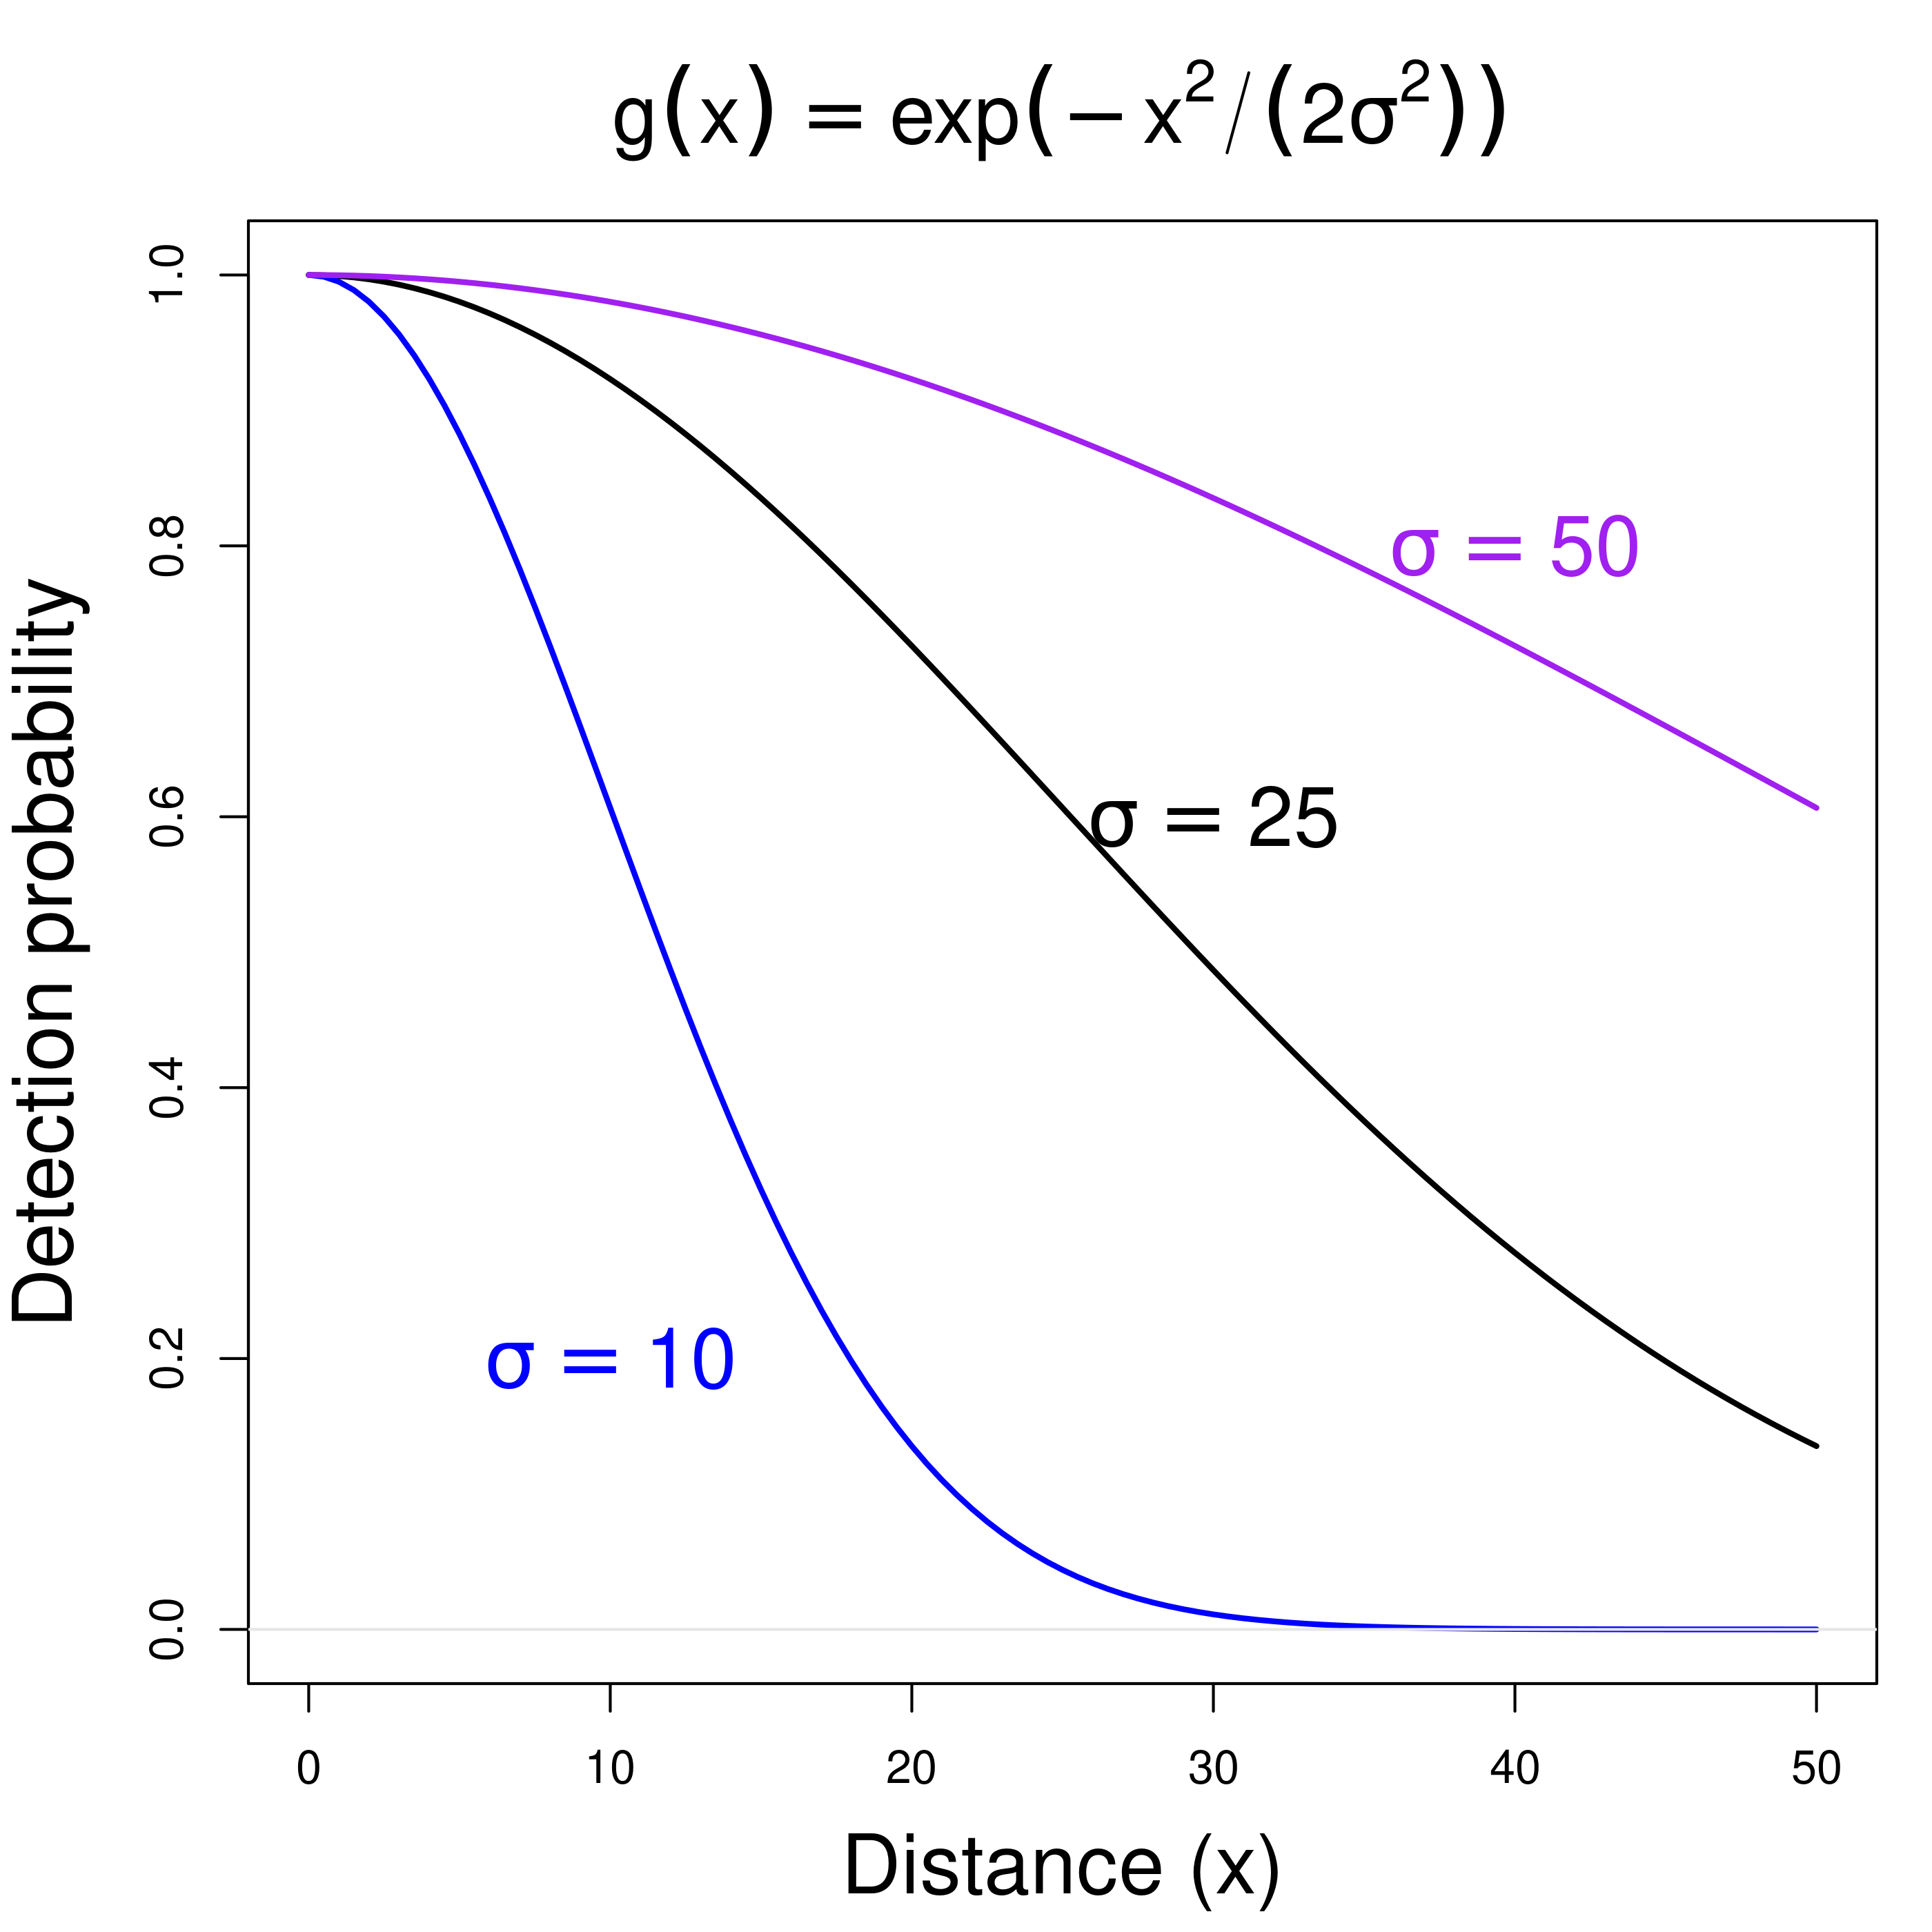
\includegraphics[width=7cm]{figs/detfun2}
\end{center}
\end{frame}



\begin{frame}
  \frametitle{Computing $\bar{p}$, average detection probability}
\begin{center}
  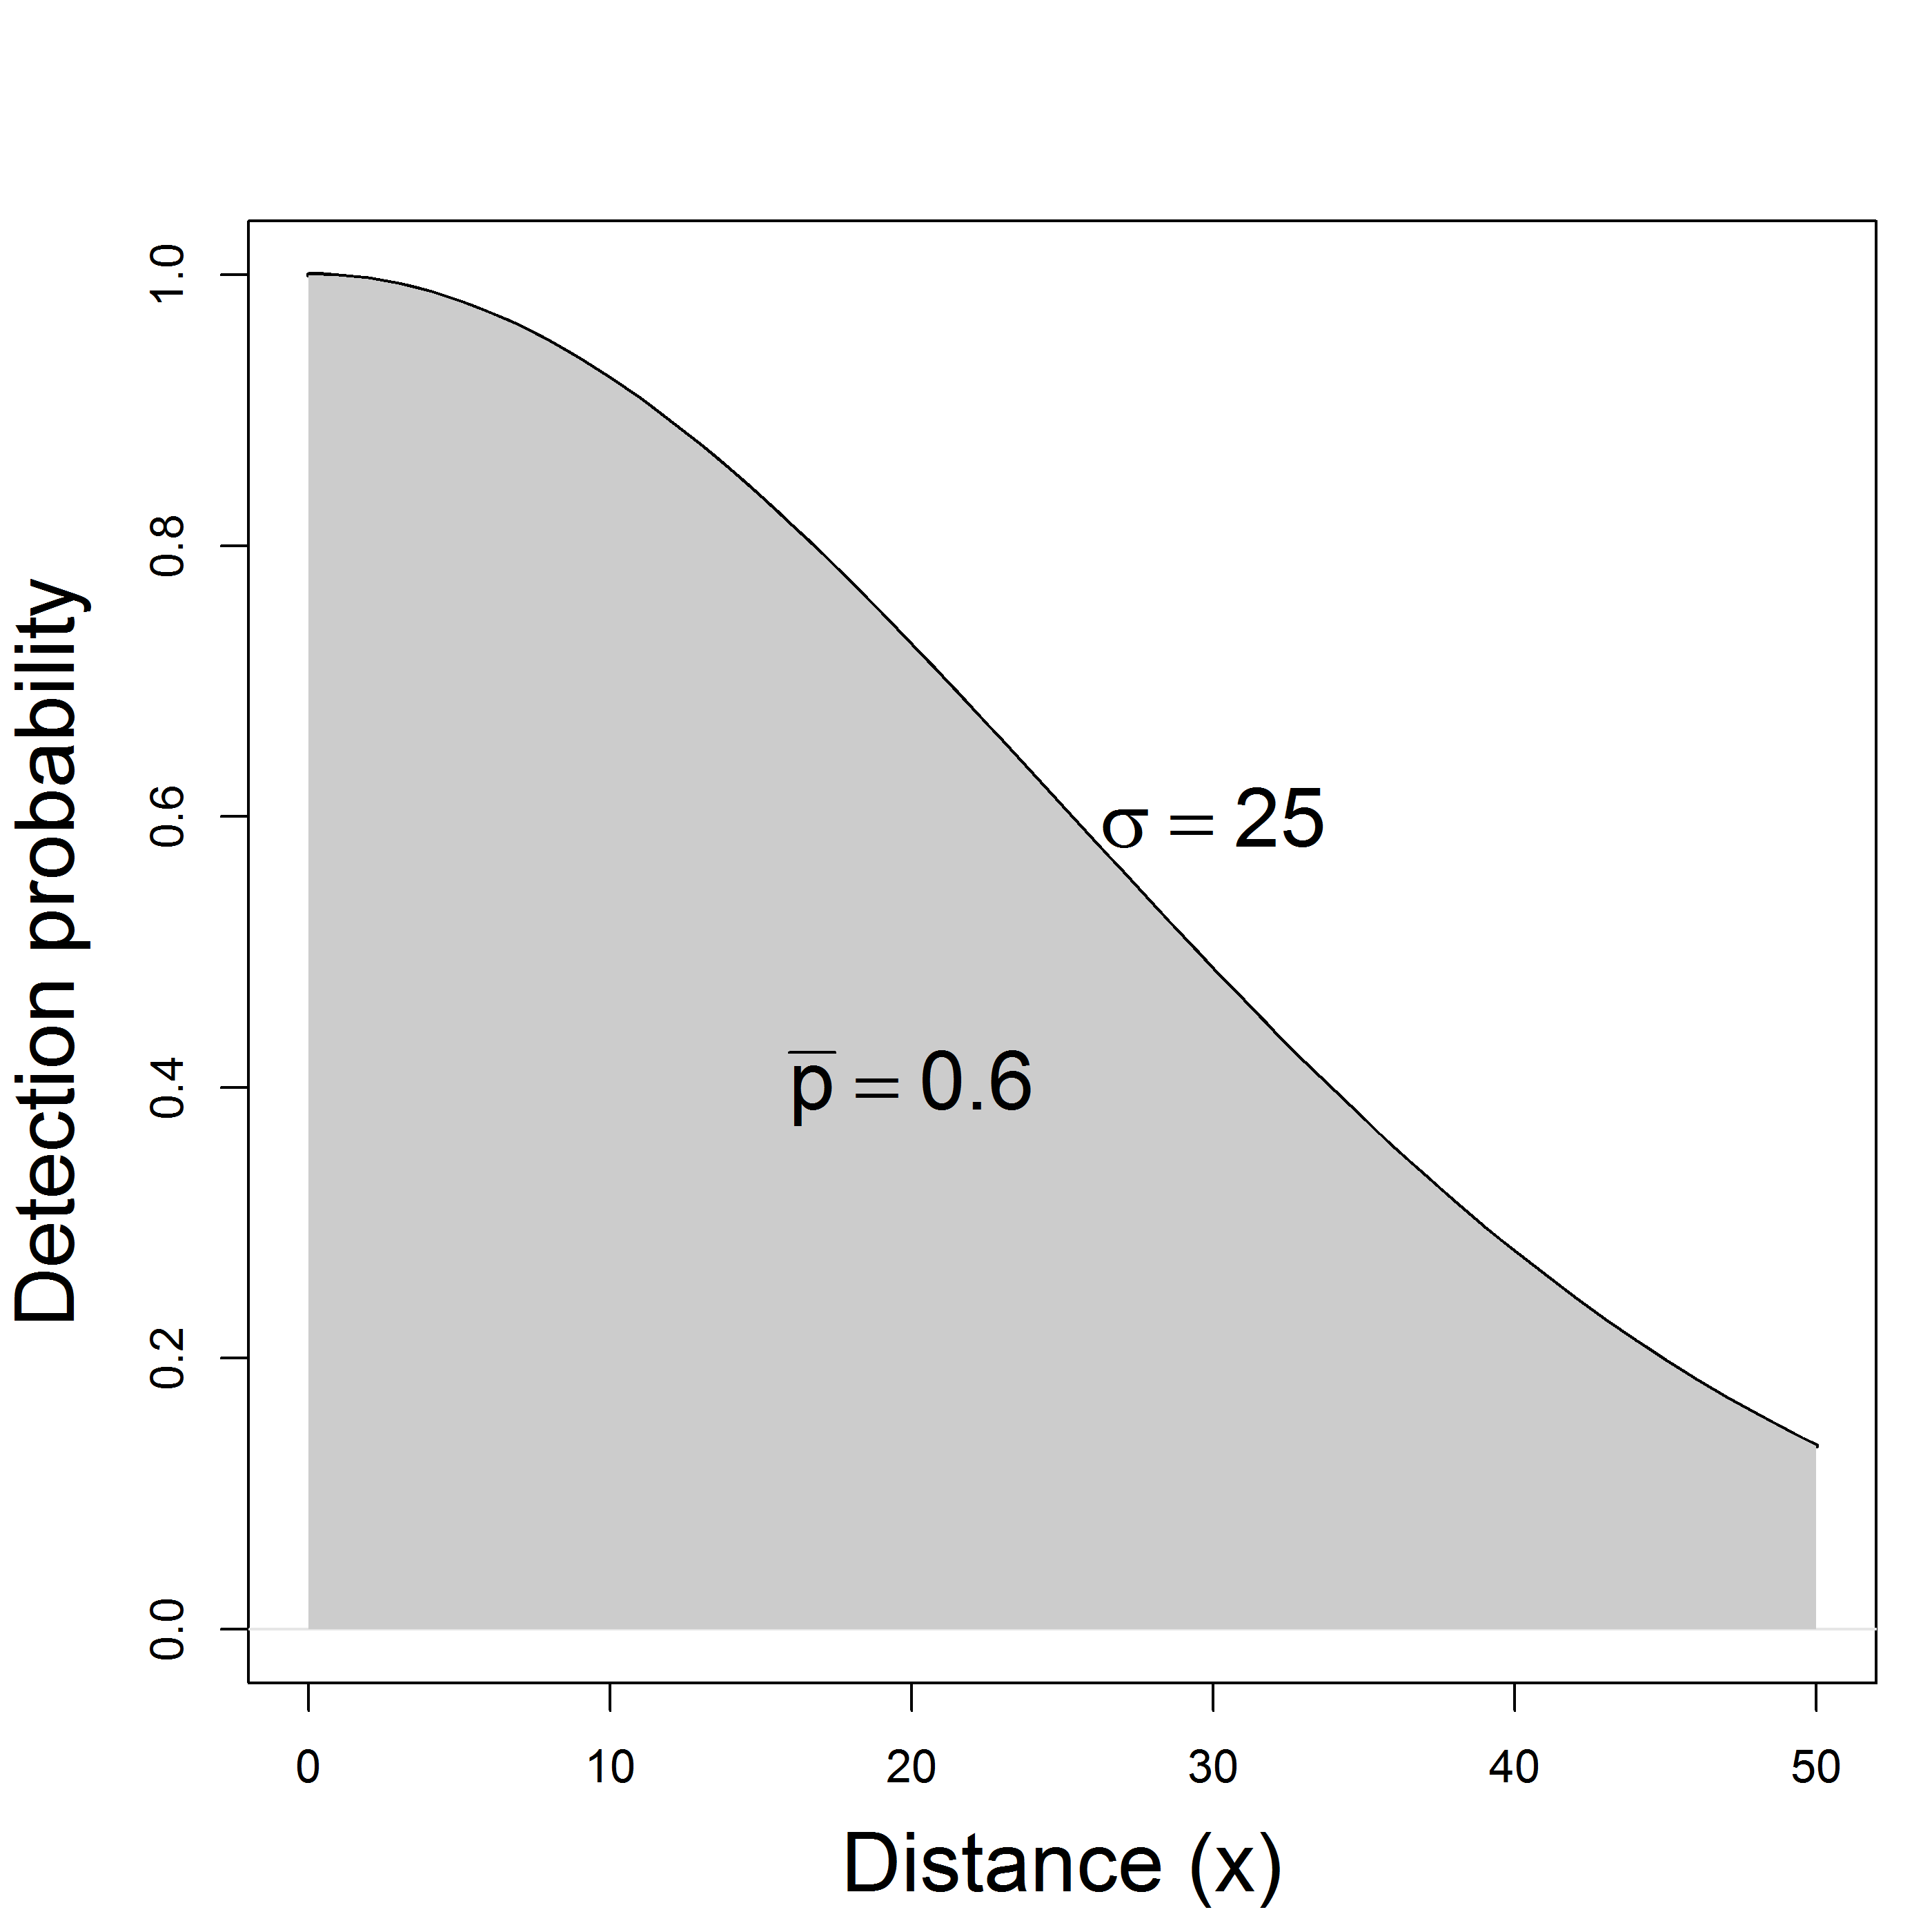
\includegraphics[width=7cm]{figs/detfun3}
\end{center}
\end{frame}




\begin{frame}
  \frametitle{Computing $\bar{p}$, average detection probability}
\begin{center}
  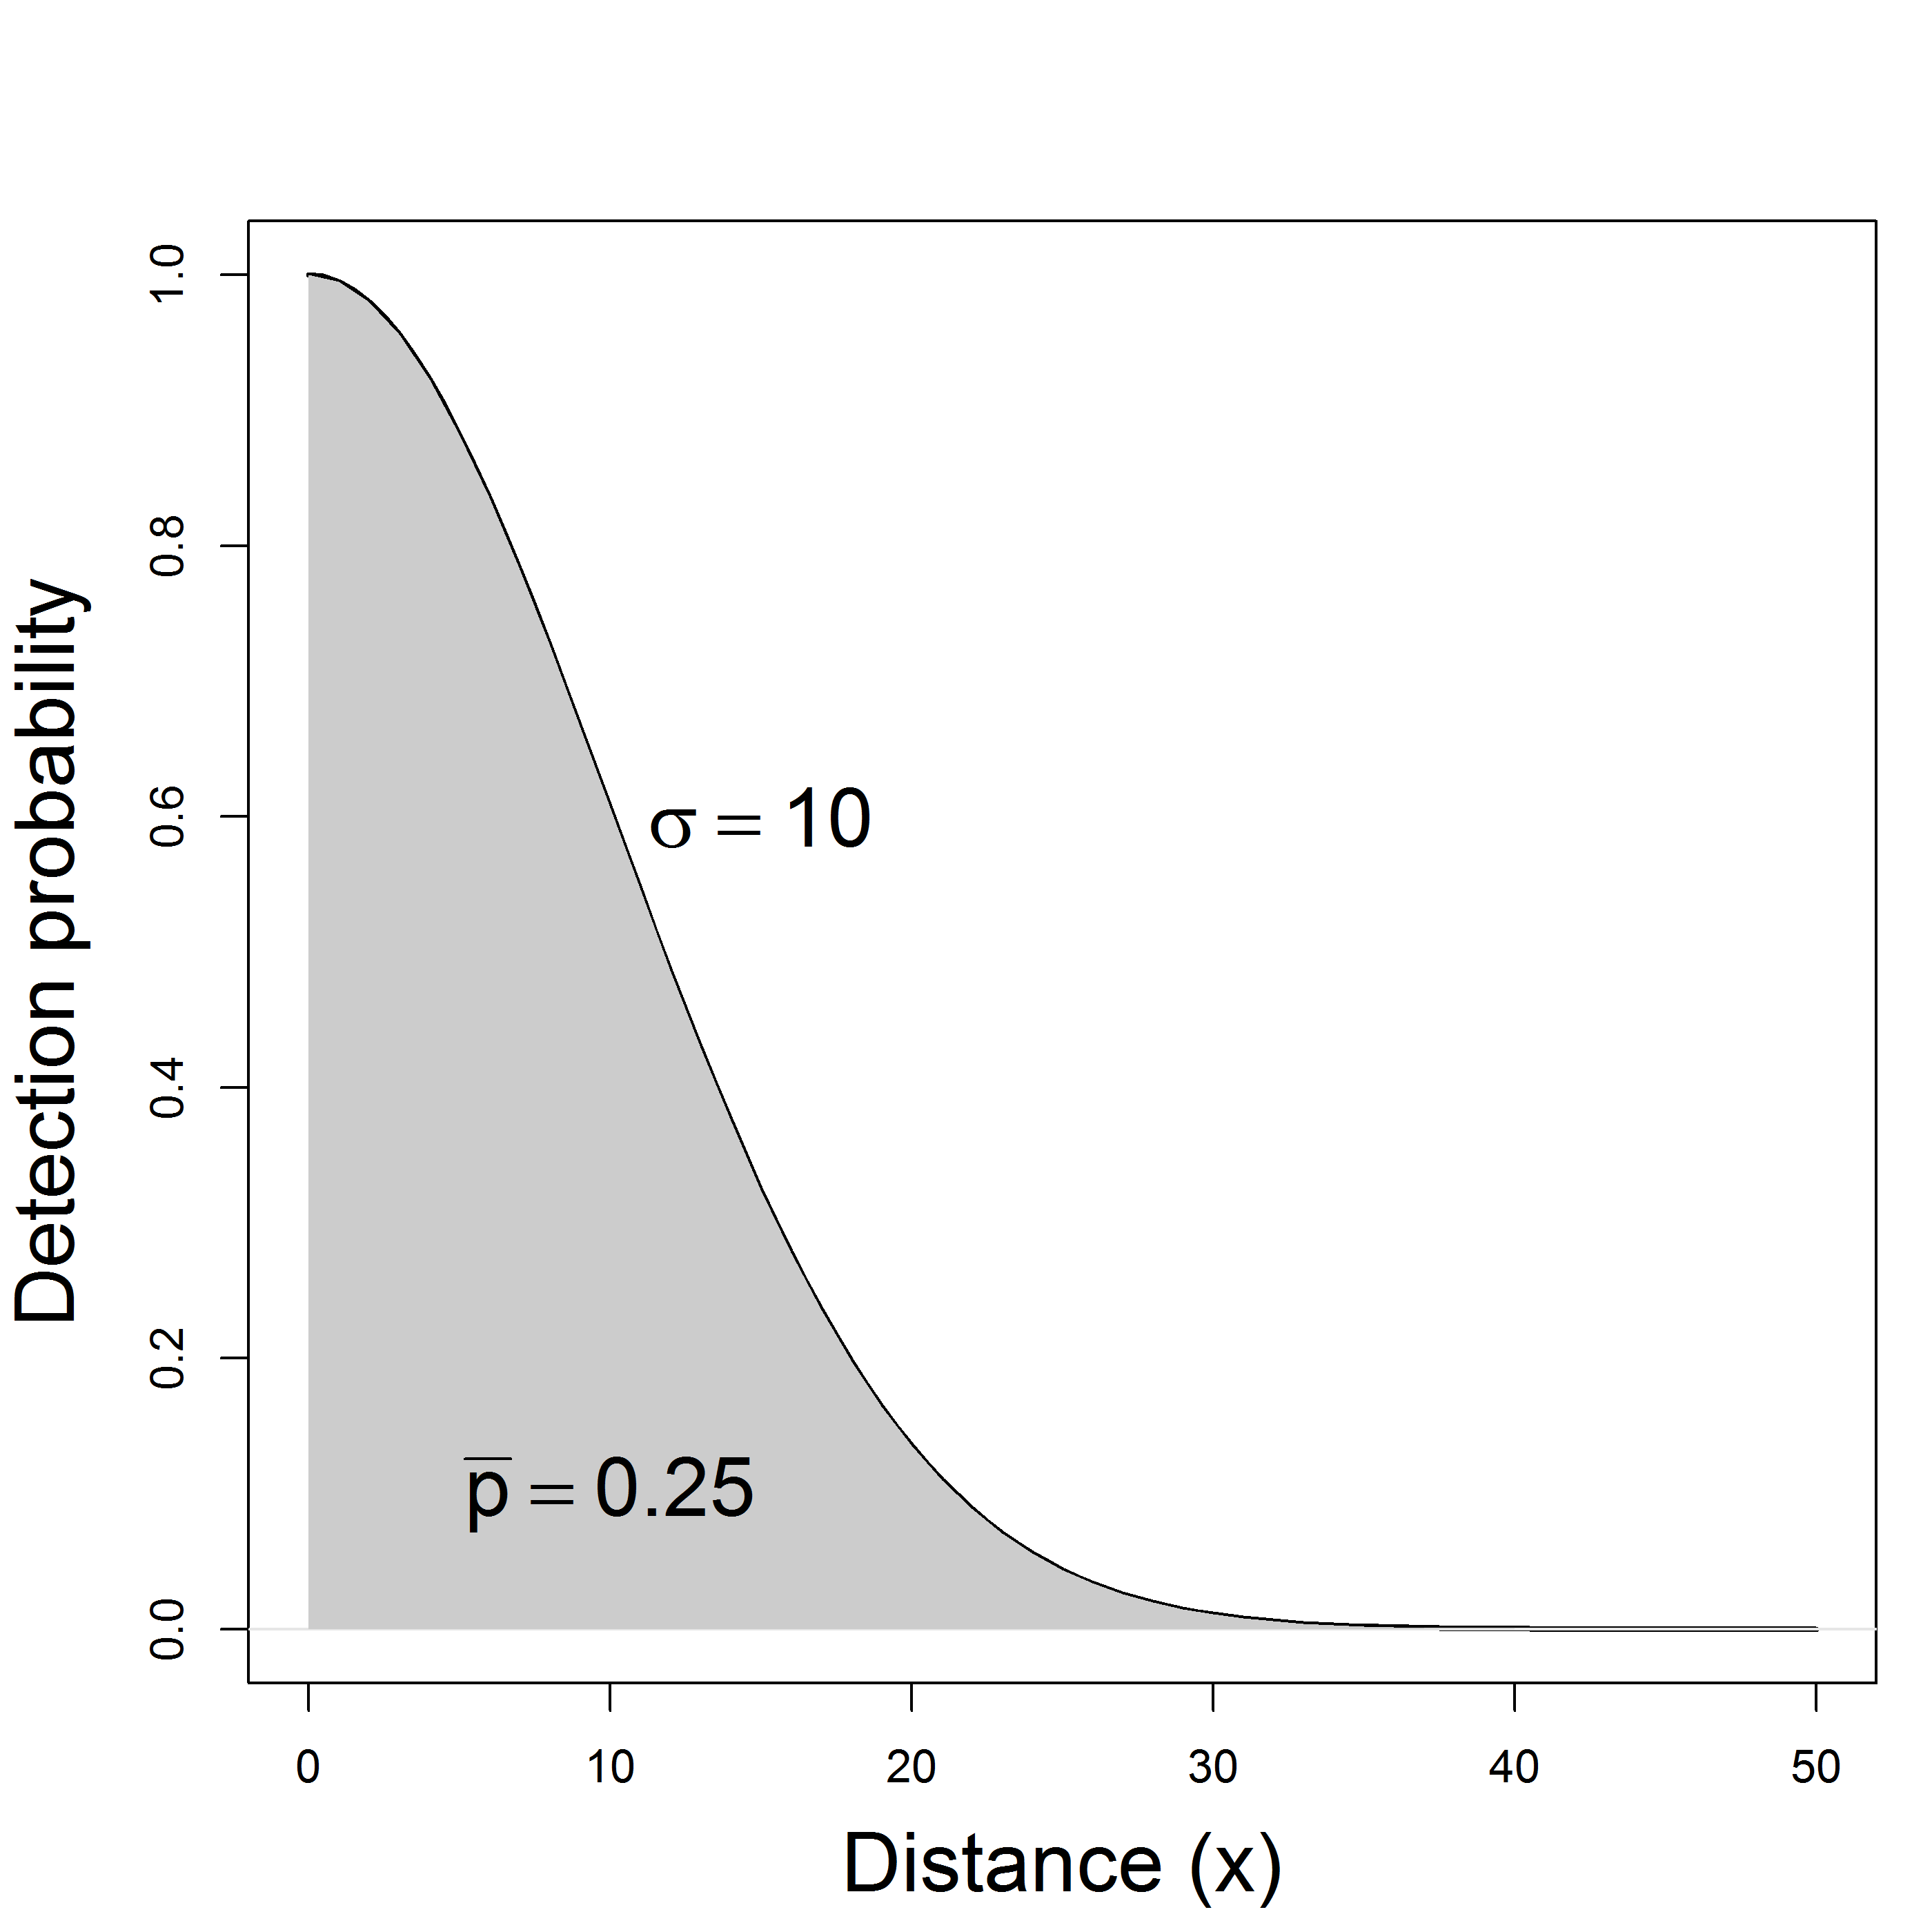
\includegraphics[width=7cm]{figs/detfun4}
\end{center}
\end{frame}









% \begin{frame}
%   \frametitle{Estimation}
% %  \begin{block}{\bf Impose a Model}
% %    \begin{gather*}
% %      C \sim \mathrm{Binomial}(N, p)% \\
% %      \mathrm{or} \\
% %      C \sim \mathrm{Binomial}(N, p_p p_a)
% %    \end{gather*}
% %  \end{block}
%   \begin{block}{\bf To estimate $\sigma$, we just need the
%       conditional likelihood}
%     \begin{gather*}
%       \mathcal{L}(\sigma | C) = \prod_{i=1}^C \frac{\mathrm{g}(x_i)[x_i]}{\int_0^w \mathrm{g}(x)[x]}
%     \end{gather*}
%   \end{block}
%   \pause
%   \begin{block}{Once we have $\hat{\sigma}$, we can compute $\hat{p}$
%       and $\hat{N}$}
%     \pause
%     \begin{gather*}
%       \hat{p} = \int_0^w \mathrm{g}(x) [x] \, \mathrm{d}x \\
%       % \exp(-x^2 / \hat{\sigma}^2)/w
%       \hat{N} = \frac{C}{\hat{p}}
%     \end{gather*}
%   \end{block}
% \end{frame}





%\subsection{Example}







\begin{frame}
  \frametitle{Assumptions}
  \large
  \begin{enumerate}[<+- | visible@+->][\bf (1)]%[\bf \color{PineGreen} (1)]
    \item Animals on the line are detected with certainty (i.e., $p=1$ when distance=0).
    \item Animals do not move during the survey
    \item Distance is measured accurately
    \item Transect lines are placed randomly with respect to the animals
      \begin{itemize}
        \large
        \item This ensures that individuals will be uniformly
          distributed with respect to the transect
      \end{itemize}
    \item Detections (of individuals or groups) are independent of one another
  \end{enumerate}
\end{frame}





% \begin{frame}
%   \frametitle{If detection is perfect}
%   \[
%     \hat{D} = \frac{n}{2Lw}
%   \]
% \end{frame}


% \begin{frame}
%   \frametitle{If detection probability decreases with distance}
%   \[
%     \hat{D} = \frac{n}{2L\hat{\mu}}
%   \]
% \end{frame}




\section{Point transects}





\begin{frame}
  \frametitle{Point transects}
  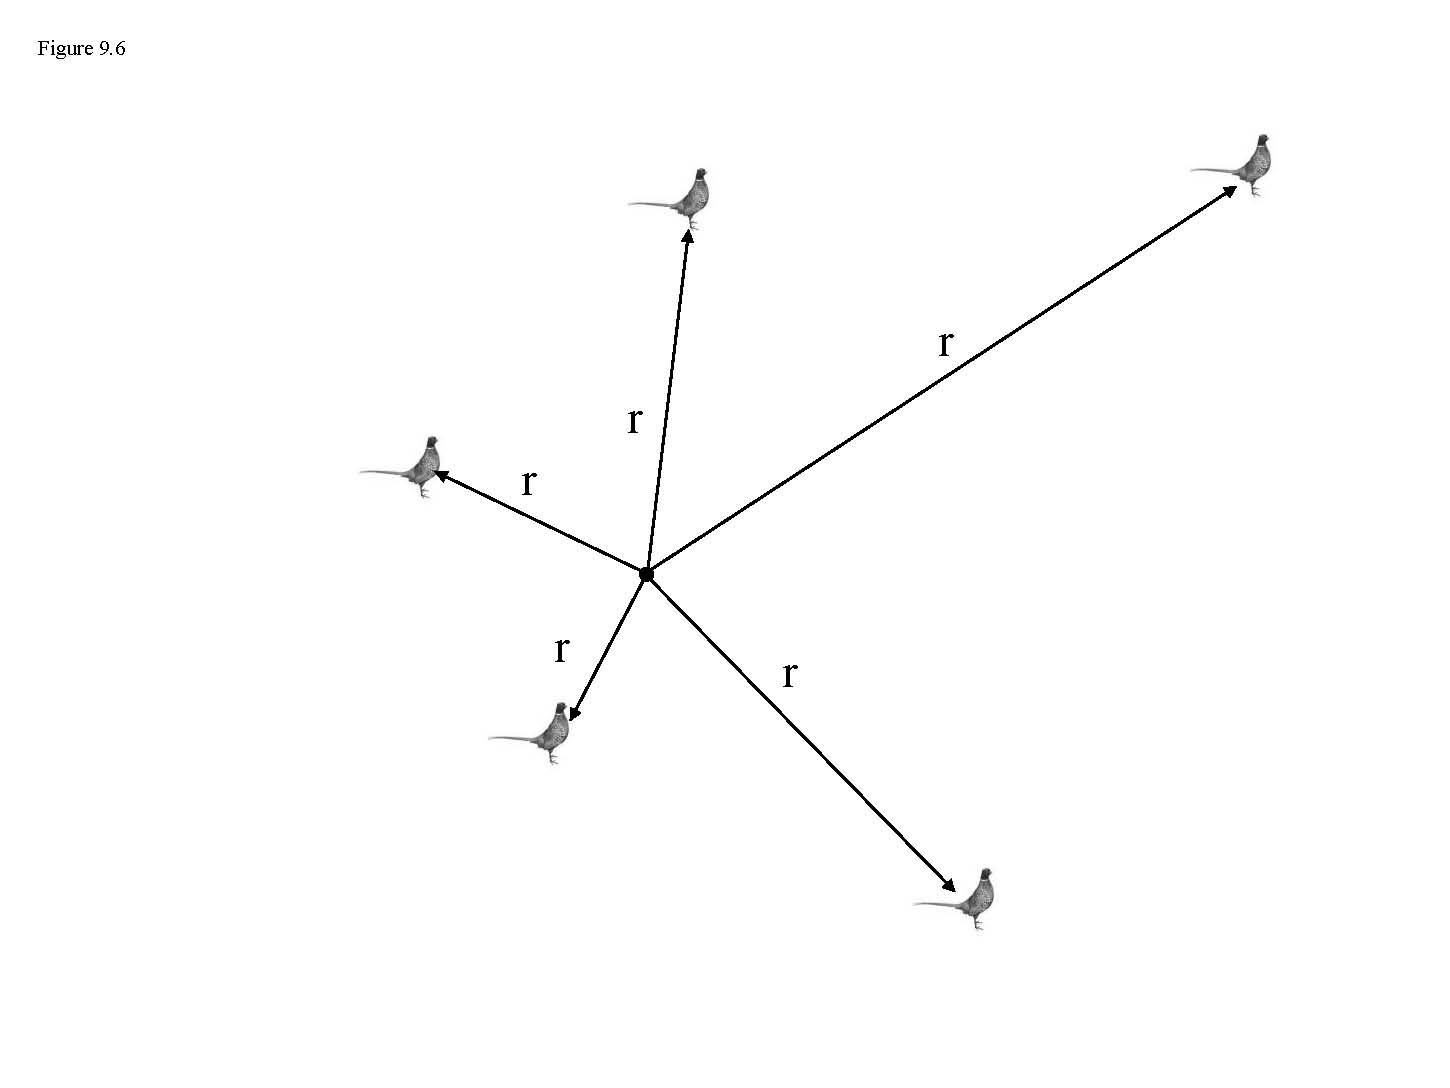
\includegraphics[width=\textwidth]{figs/fig9-8}
\end{frame}



% \begin{frame}
% \frametitle{Point transects}
% \begin{center}
%   \includegraphics[width=7cm]{figs/inplot1}
% \end{center}
% \end{frame}




% \begin{frame}
% \frametitle{Point transects}
% \begin{center}
%   \includegraphics[width=7cm]{figs/detect1}
% \end{center}
% \end{frame}







%\begin{comment}

\begin{frame}
  \frametitle{Differences between point vs line transects}
%  \begin{columns}
%    \begin{column}{5cm}
%      \begin{block}
  \large
  {We still use the same type of detection function (half-normal,
    hazard, etc.) \par}
  \pause
  \vfill %\vspace{0.3cm}
  {We don't expect a ``flat'' histogram of distances when
    $\bar{p}=1$. Why? \par}
  \pause
  \vfill %\vspace{0.3cm}
  {Because there is a slim chance of an individual being
    close to point} \par
%  \begin{itemize}
%    \item $\mathrm{g}(x)$ is the same (half-normal, hazard, etc...)
%    \item But individuals are not
%  \end{itemize}
%    \end{block}
%    \end{column}
%    \pause
%    \begin{column}{5cm}
%      \begin{center}
%        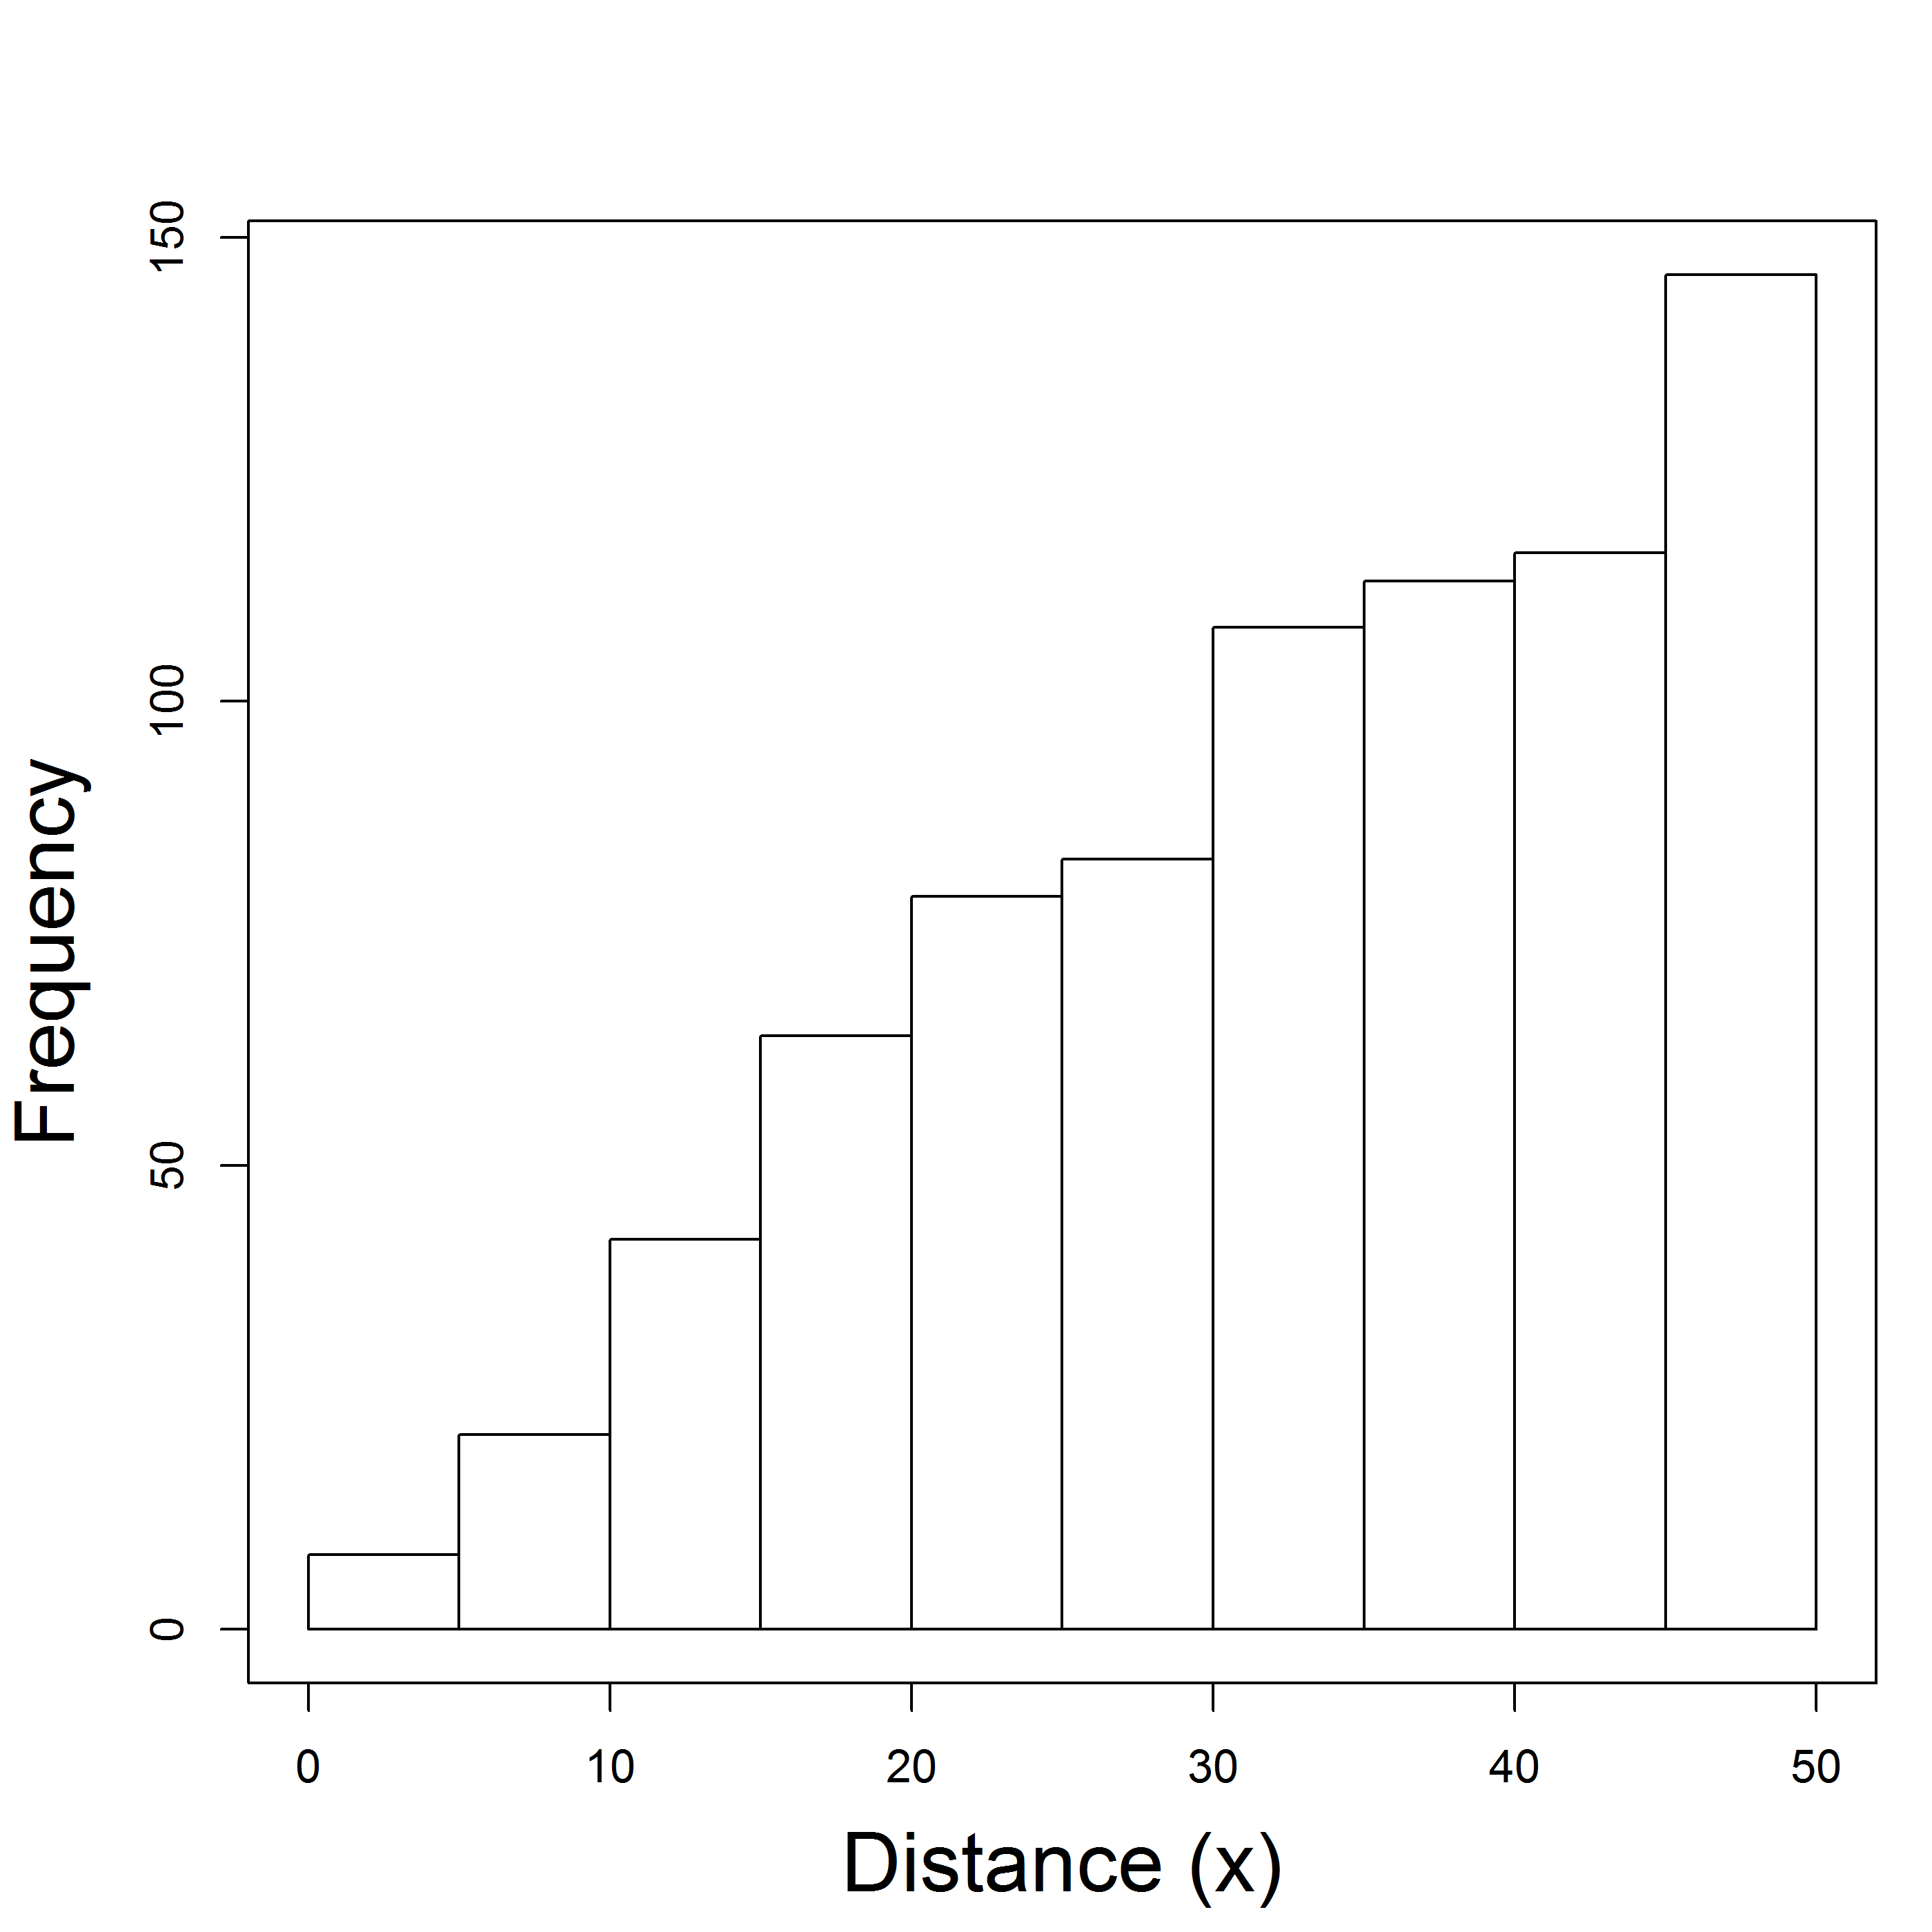
\includegraphics[width=4cm]{figs/detfun5}
%      \end{center}
%    \end{column}
%  \end{columns}
\end{frame}

%\end{comment}




% \begin{frame}
% \frametitle{Point transects}
% \begin{center}
%   \includegraphics[width=7cm]{figs/design1}
% \end{center}
% \end{frame}





\begin{frame}
  \frametitle{Point Transects. $\bar{p}=1$}
  \centering
  When average detection probability is 1, the histogram of distances
  will look like this because there is more area (and hence more
  individuals) far from the point. \\
  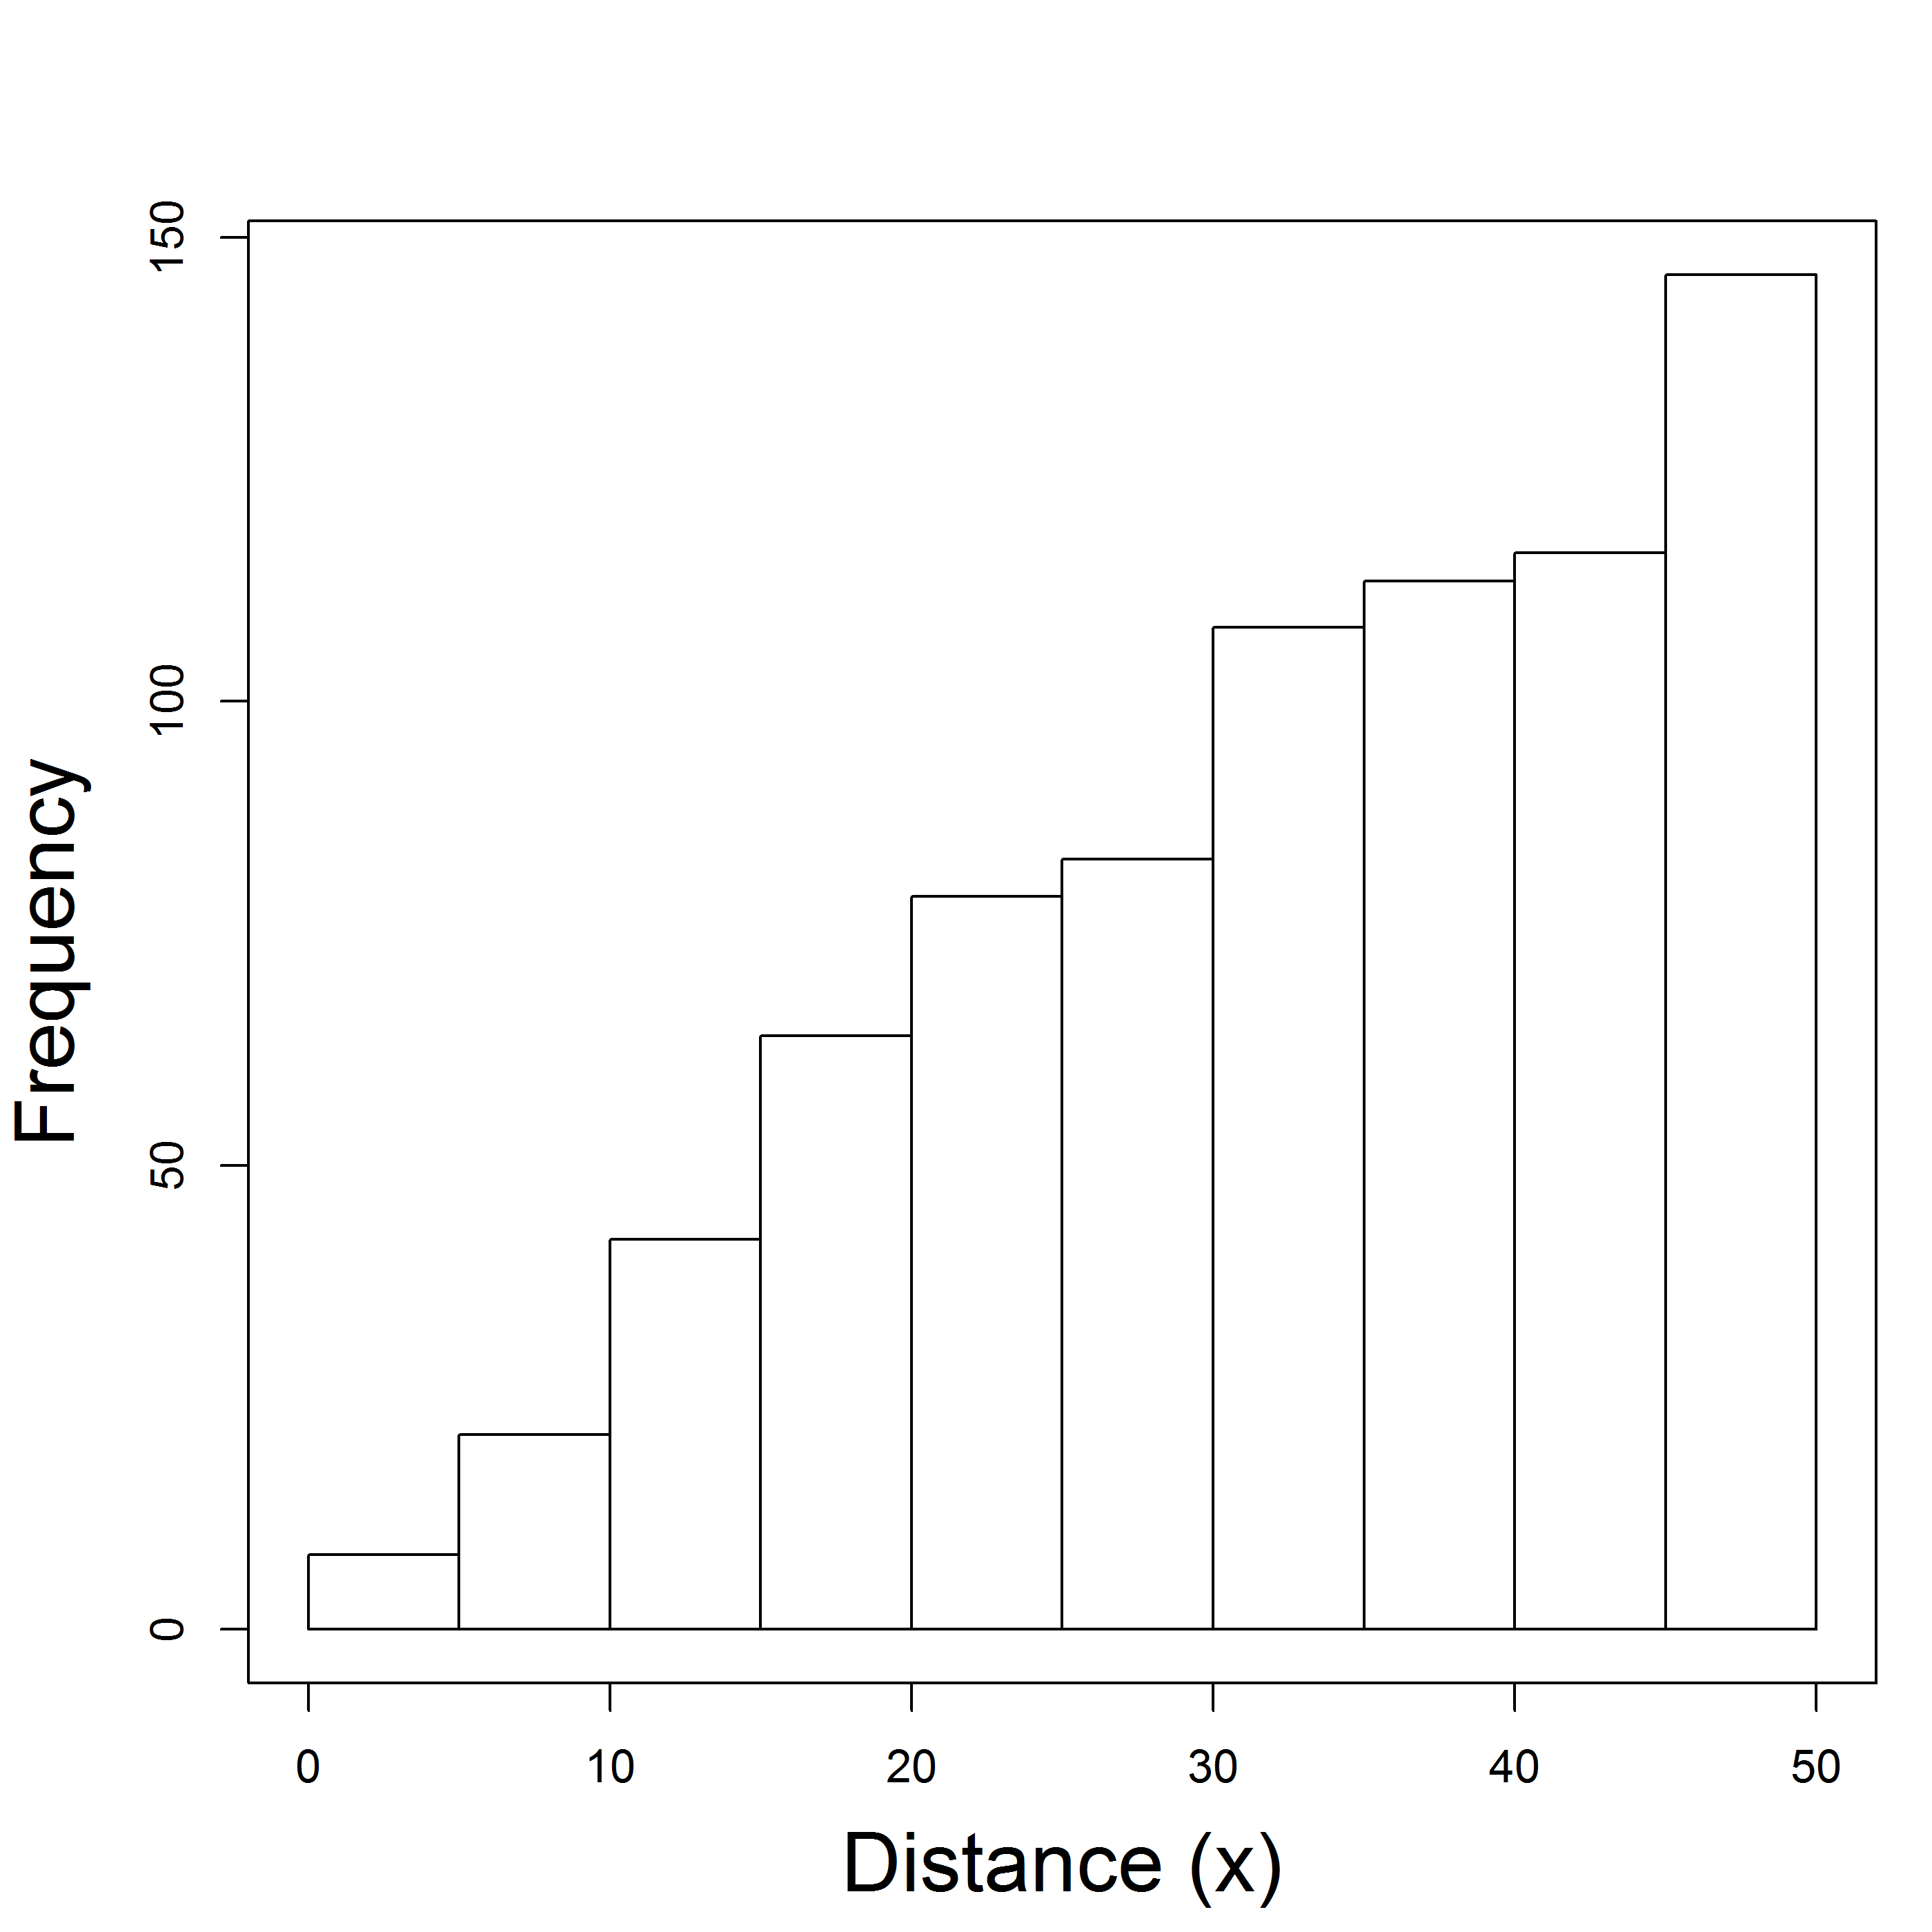
\includegraphics[width=6cm]{figs/detfun5} \\
\end{frame}




\begin{frame}
  \frametitle{Point Transects. $\bar{p} < 1$}
\begin{center}
  If average detection probability is less than 1, the histogram will
  increase and then decline. \\
  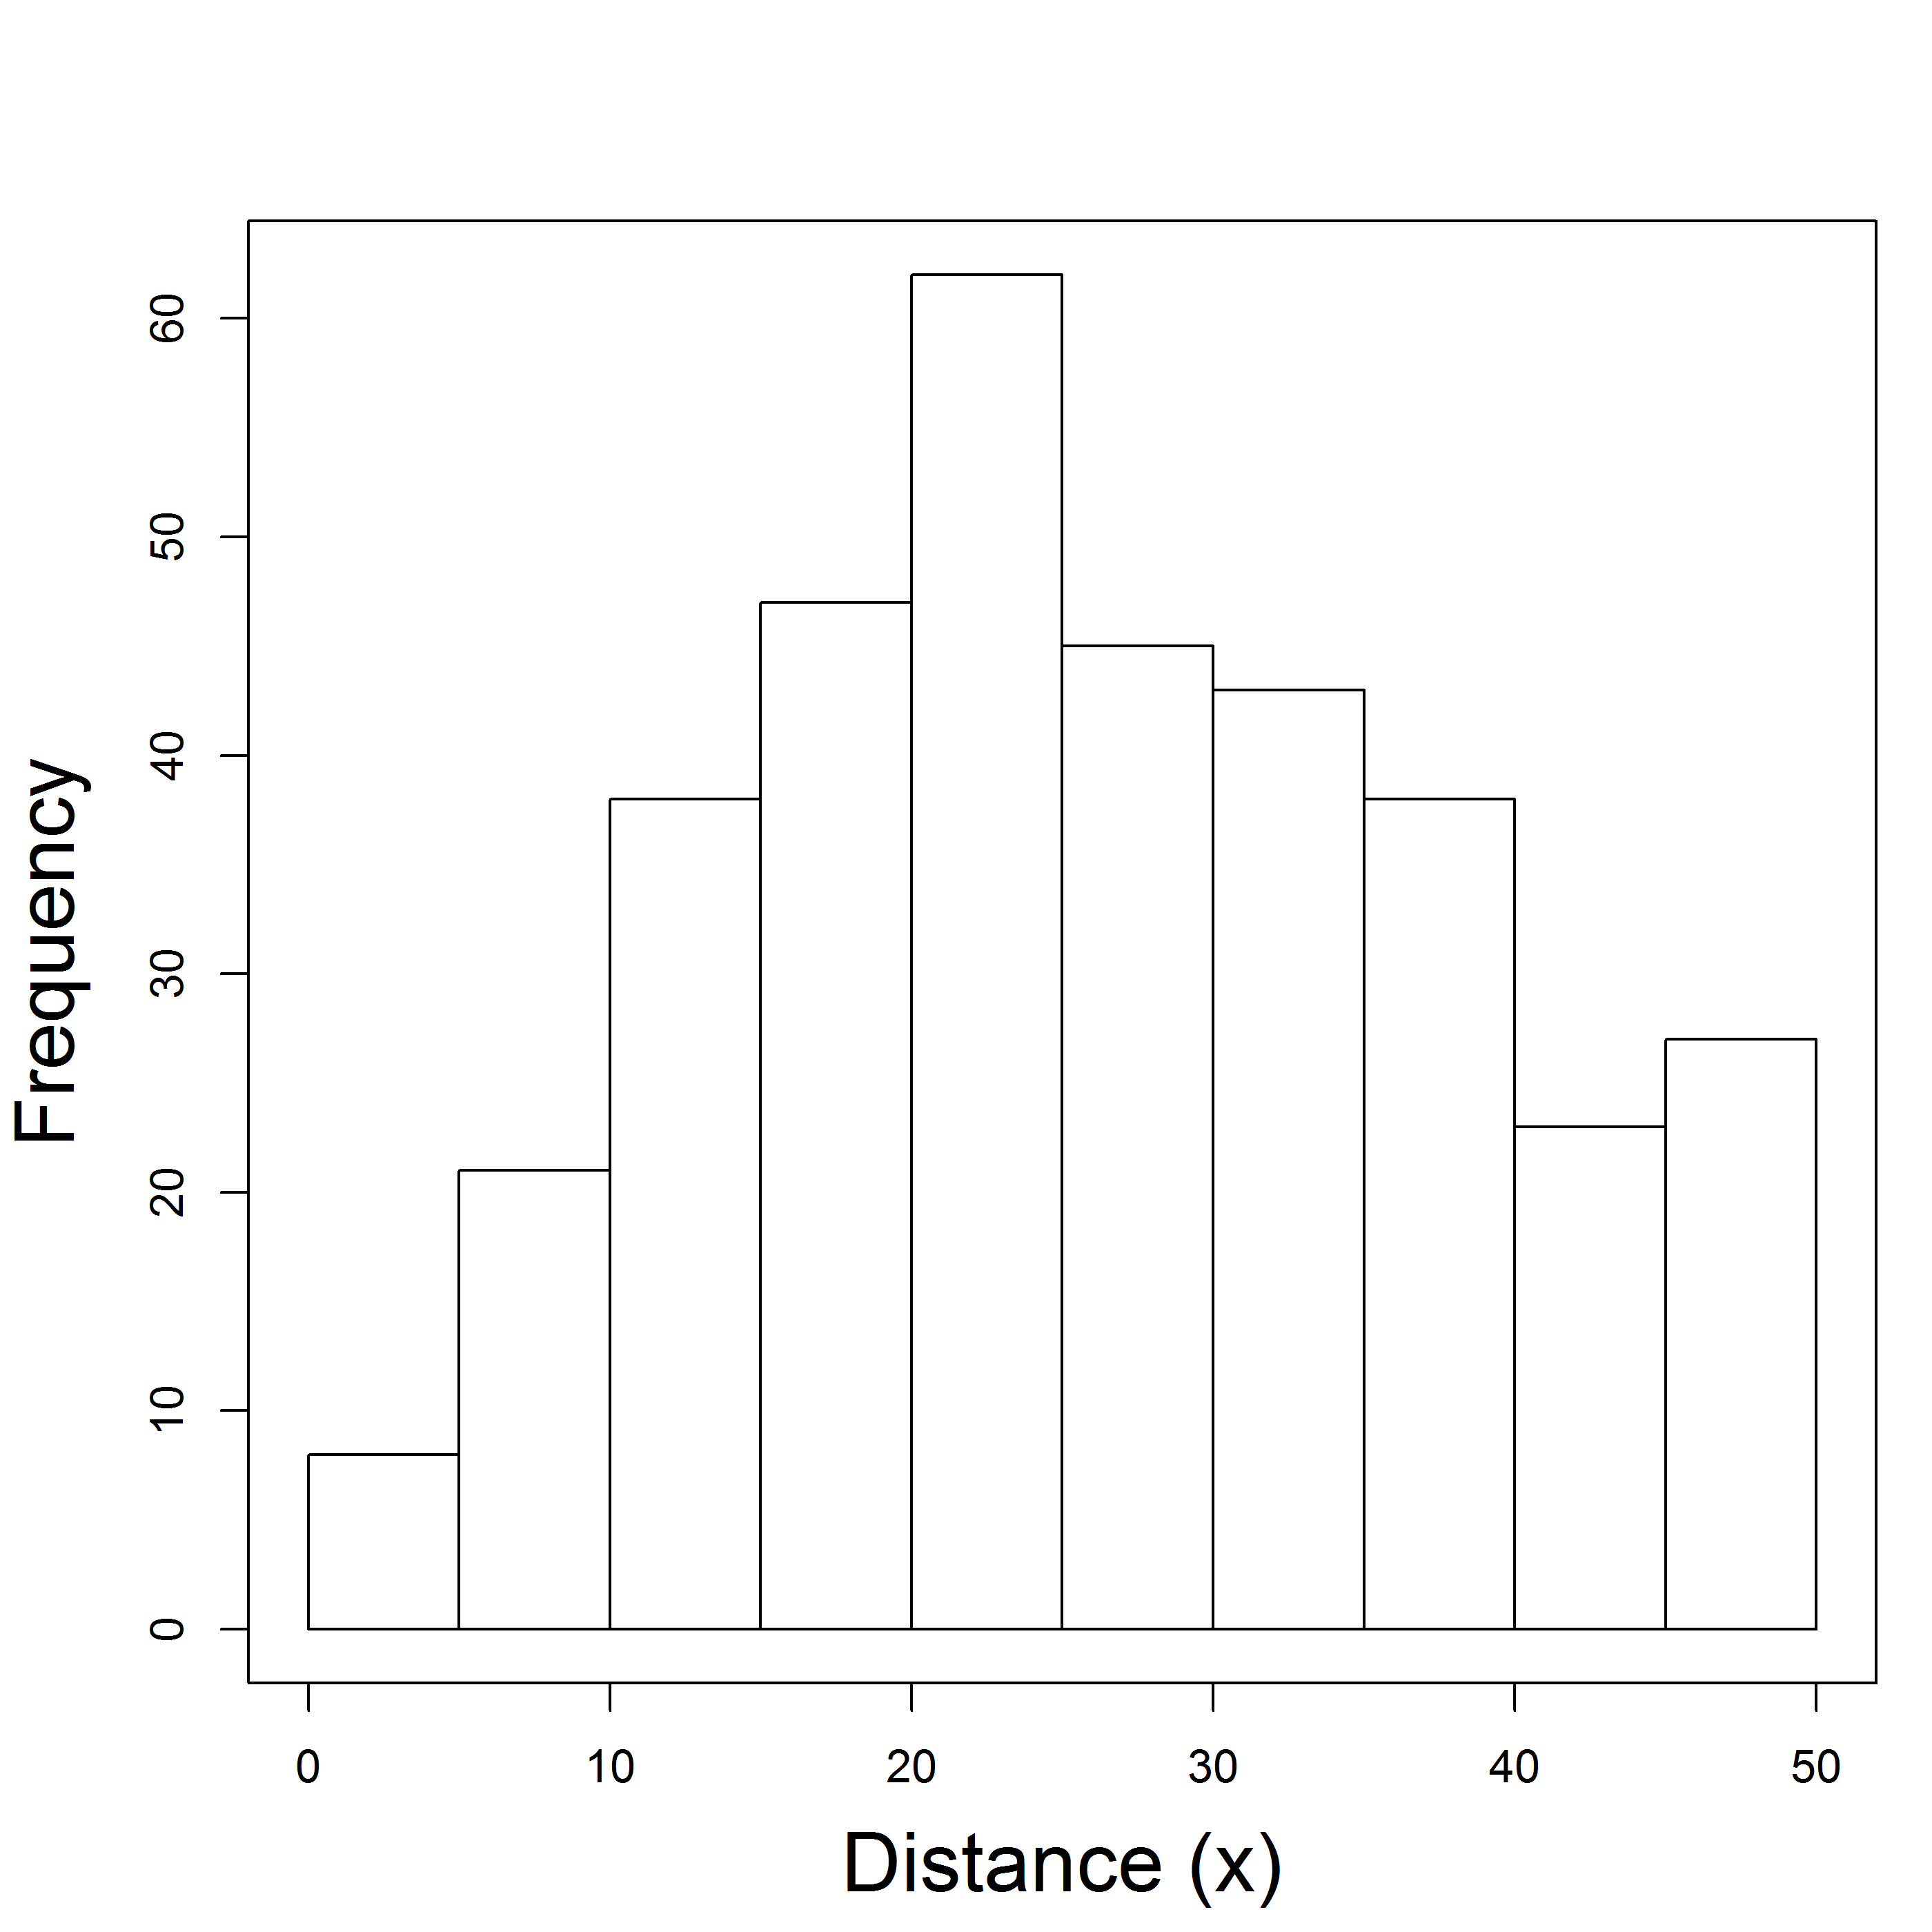
\includegraphics[width=6cm]{figs/detfun6}
\end{center}
\end{frame}




\begin{frame}
  \frametitle{Point Transects. $\bar{p} < 1$}
\begin{center}
  The fitted curve will look like this \\
  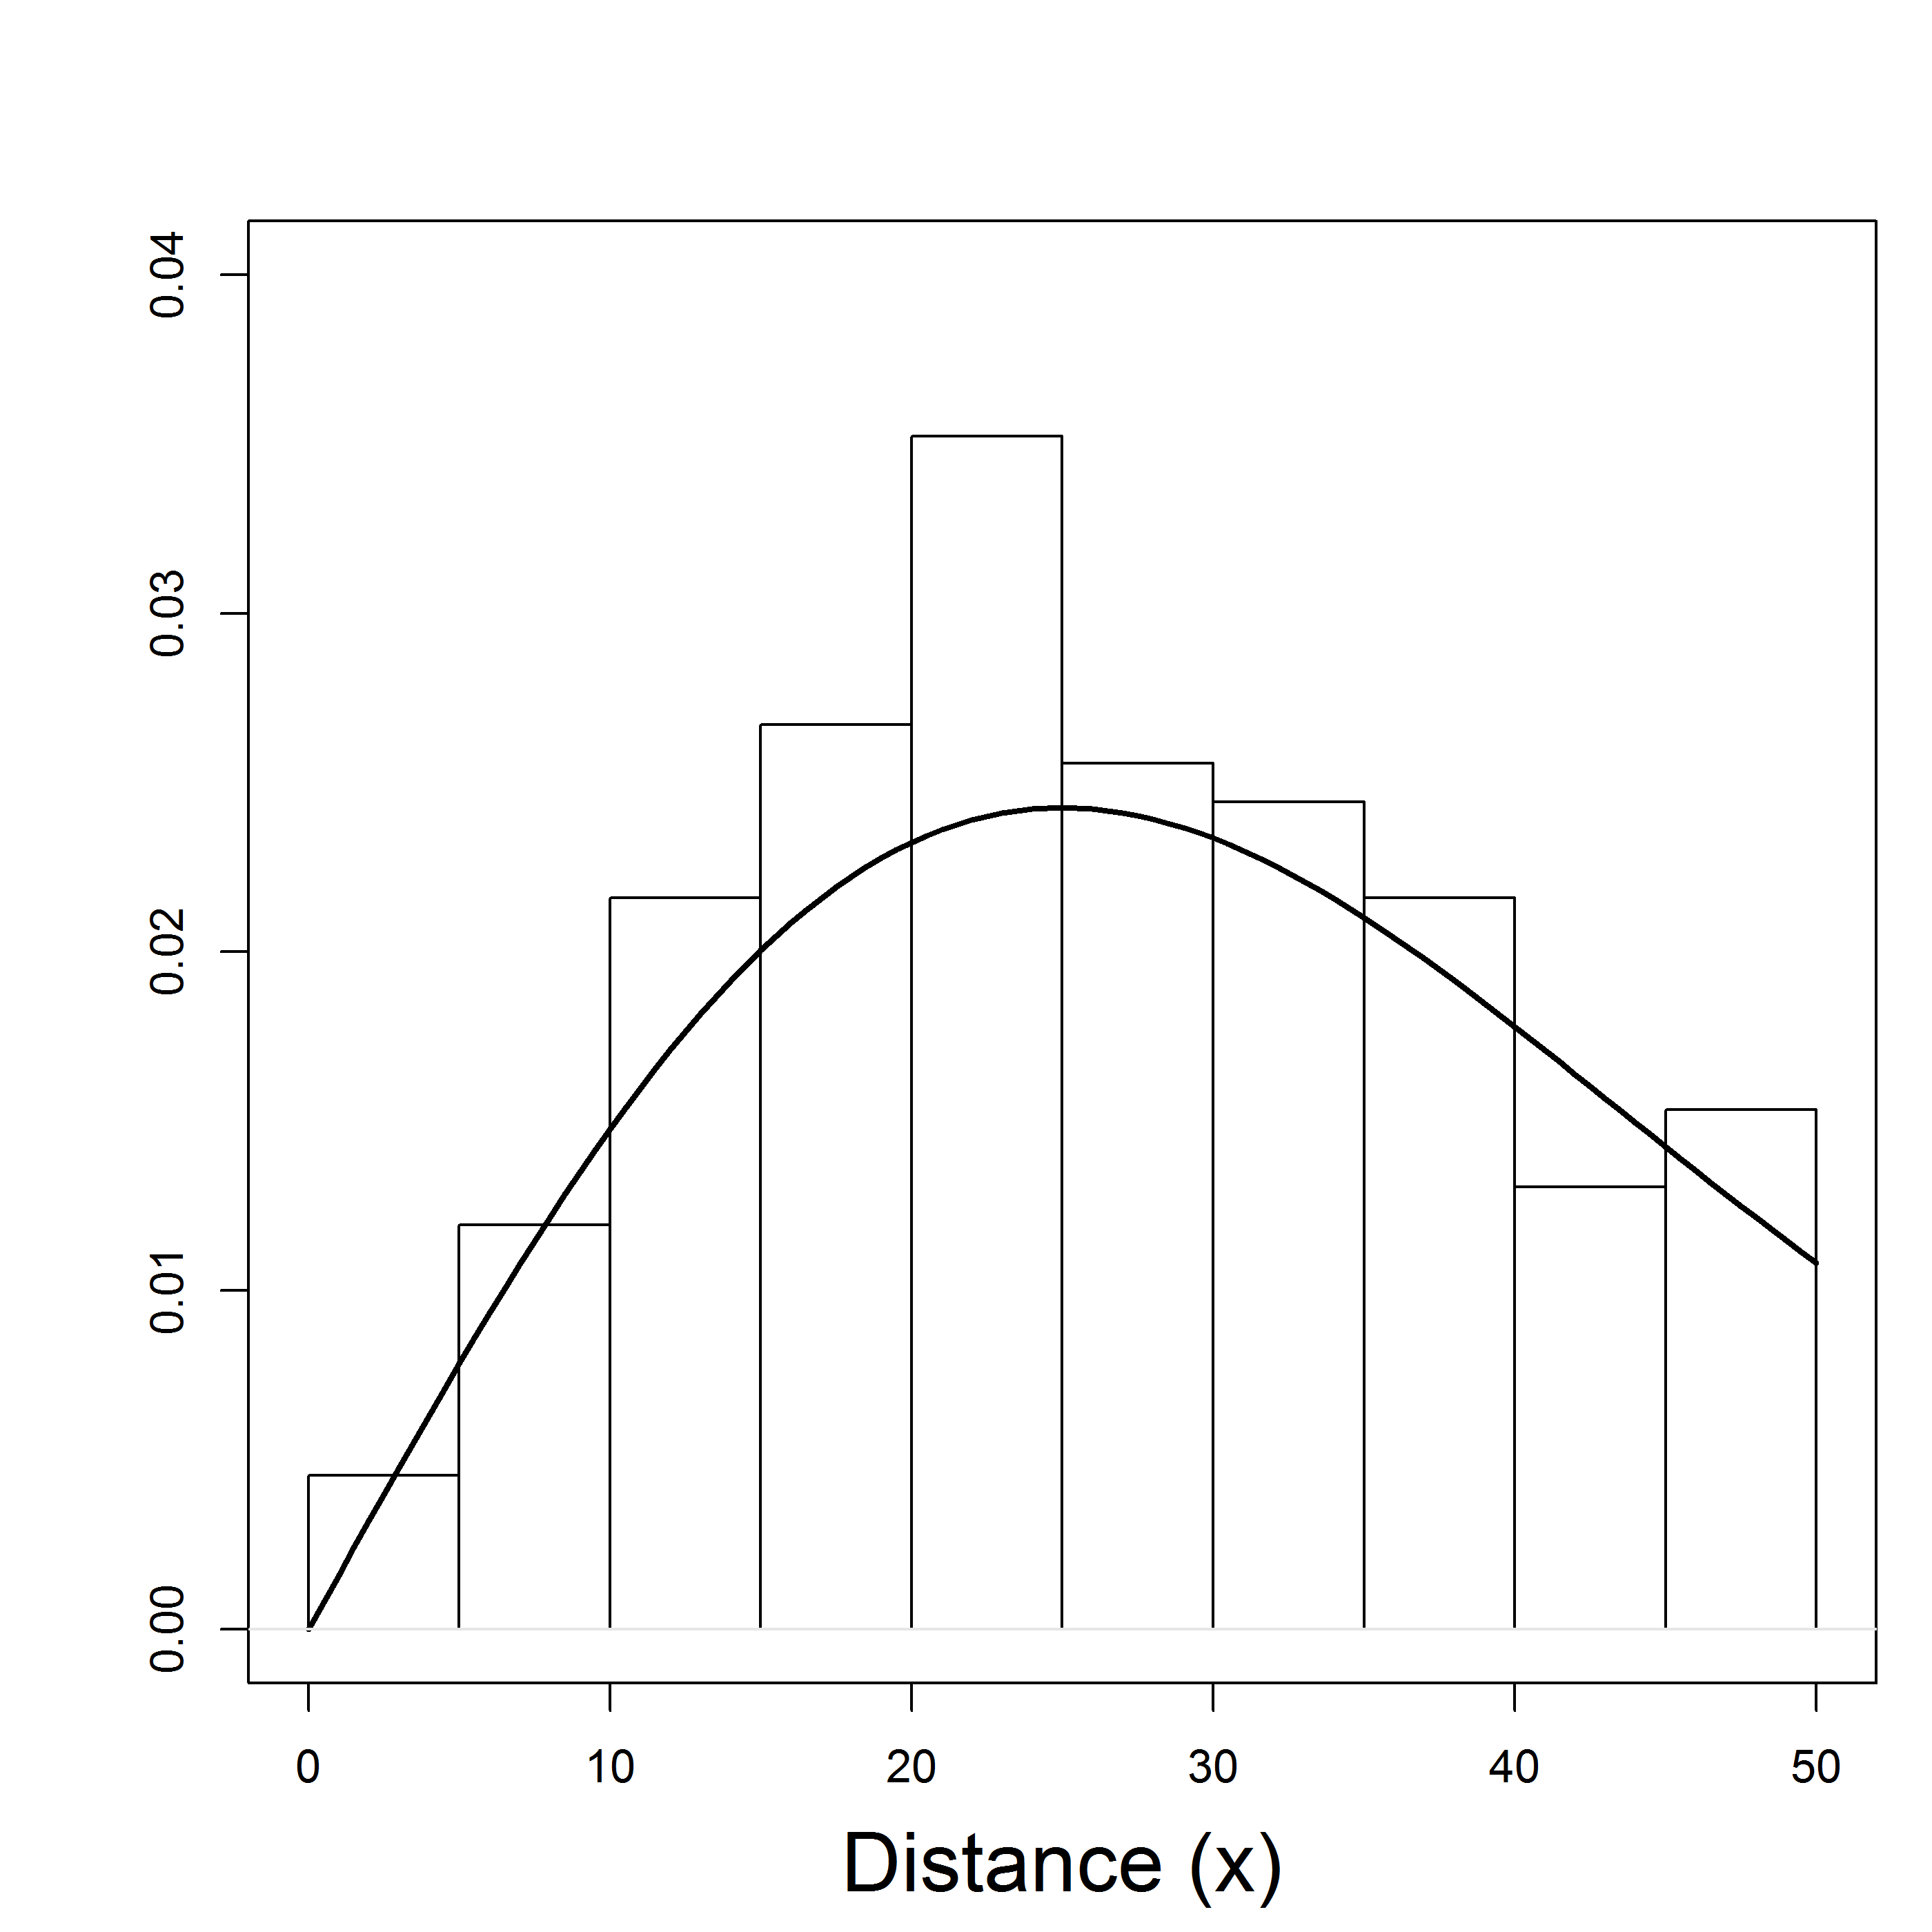
\includegraphics[width=6cm]{figs/detfun7}
\end{center}
\end{frame}







%\section{Summary}




\begin{frame}
  \frametitle{Assignment}
  \Large
  \begin{center}
    Read Chapter 10 -- Capture-Mark-Recapture
  \end{center}
\end{frame}




\end{document}



